


In this section, we present the results obtained from multiple conducted experiments of the overlay protocol against state-of-the-art baselines. These experiments aimed at testing: (1) the cost of establishing/maintaining the overlay networks for each protocol; (2) testing the establised networks' efficiency (according to latency); and (3) finally, testing demmons' message dissemination capabilities against the same baseline set of baseline protocols, executing two distinct dissemination protocols. We now begin by providing a brief discussion of the protocols and parameters used for conducting the experiments

\subsection{Baselines and configuration parameters}

The chosen protocols (discussed in further detail in section \ref{sec:topology_management}) to perform the overlay protocol network establishment and construction comparison were: (1) \textbf{Hyparview} \todo{ref}, which is a protocol that builds a non-structured overlay network using a fixed-sized view materialized by active bidirectional TCP connections (these connections also used for fault tolerance); the second baseline protocol is \textbf{X-Bot} \todo{ref}, which is a protocol that essentially employs Hyparview to establish the initial overlay structure, and optimizes (whenever possible) the overlay network according to a configurable heuristic. These optimizations are performed via gossip mechanisms and improve active connections' costs. It is important to mention optimizations are performed in such a way that maintains the guaranteed established by the Hyparview protocol, through a two-step exchange of the active connections of two distinct pairs of nodes, in a coordinated manner. The third implemented baseline protocol was \textbf{Cyclon} \todo{ref}, which is an overlay protocol that materializes a network composed by asymetric links via periodic exchanges of node pointers with a configurable age. The last implemented baseline was \textbf{T-Man} \todo{ref}, which is a protocol that iteratively builds on an existing set of nodes to build a new, optimized, set of nodes. These optimizations are performed iteratively by each node in the system such that a configurable cost function  (defined a priori) gets minimized. In order to feed the initial view for this overlay protocol, we employed the Cyclon protocol, which is why in the evaluation results for this protocol are labeled as ``Cyclon T-Man''. All of the described baseline protocols were, for comparativeness, implemented using the GO-BABEL framework (described in section \ref{sec:Node-Watcher}), and, as GO-BABEL only provides unidirectional connections, protocols which require bidirectional connections (hyparview, x-Bot and deMMon) were added periodic mechanisms to ensure that the two connections were established.


The utilized parameters for the protocols were adjusted to attempt to perform a fair comparison of the evaluated protocols, which are displayed in table \ref{table:proto_test_params}, the first column called ``VSizeMax'' represents the maximum size of the active view, which in most protocols was set as 5 except for cyclon where it was set as 7 as it is the only protocol without a backup secondary view. In the case of deMMon, this value represents the maximum number of children per node. The second parameter, denominated ``VSizeMin'', corresponds to the minimum number of children for each node in deMMon. The third parameter, titled ``PVSizeMax'' corresponds to the maximum size of the passive view, which is set as 25 for deMMon, hyparview and X-BOT, and set as 7 for the case of Cyclon T-Man (which corresponds to the size of the cyclon view, running in the background, to feed its initial view). The next parameter, called ``Shuffle'', corresponds to each protocols' shuffle mechanism, which is configured to execute every 5 seconds for all protocols. Following, we have the ``PWRL'' parameter, which corresponds to the TTL of the random walks for each protocol that has a random walk mechanism. The last parameter worth mentioning is the ``$\delta$T'' parameter, which corresponds to the minimum latency improvement for both X-Bot to perform active view exchanges and for deMMon to make opportunistic improvements. Some parameters such as timeouts and the duration of some periodic procedures were omitted, however all timeouts (e.g. timeouts for dialing nodes, receiving message responses, among others) are lower than 5 seconds, and all periodic mechanisms are executed with a frequency lower than 15 seconds.

\todo{pode haver mais parametros / talvez meter uma tabela completa em anexo?}
\begin{table} \label{table:proto_test_params}
    \caption{Membership evaluation: protocol configuration parameters}
    \scalebox{1}{
    \centering
    \resizebox{\textwidth}{!}{%
    \begin{tabular}{llllllllllll}
                & VSizeMax & VSizeMin & PVSizeMax & Shuffle $\delta$T (s) & PRWL & ARWL & ka & kp & improvement  $\delta$T (ms) & UN & PSL \\
                Hyparview    & 5        & -        & 25        & 5                     & 6    & 3    & 2  & 3  & -                            & -  & -   \\
                X-Bot        & 5        & -        & 25        & 5                     & 6    & 3    & 2  & 3  & 50                           & 1  & 2   \\
                Cyclon       & 7        & -        & -         & 5                     & -    & -    & -  & -  & -                            & -  & -   \\
                Cyclon T-Man & 5        & -        & 7         & 5                     & -    & -    & -  & -  & -                            & -  & -   \\
                DeMMon       & 5        & 2        & 25        & 5                     & 6    & -    & -  & -  & 50                           & -  &    
    \end{tabular}%
    }
    }
\end{table}

\subsection{Overlay construction and maintenance}

The first conducted experiment, aimed at evaluating how protocols build and maintain the overlay networks, is an experiment where different numbers of nodes join the system and remain during 25 minutes. In this experiment, we evaluate what are the properties of the built overlay networks (costs, degree distribution, among other properties) and how fast the protocol converges towards an optimized network. Finally, in order to compare the scalability, performance and fault-tolerance at multiple scales, we perform the previously mentioned experiment using network sizes of 50, 250, 500 and 750 nodes.

\begin{figure}
    \centering
    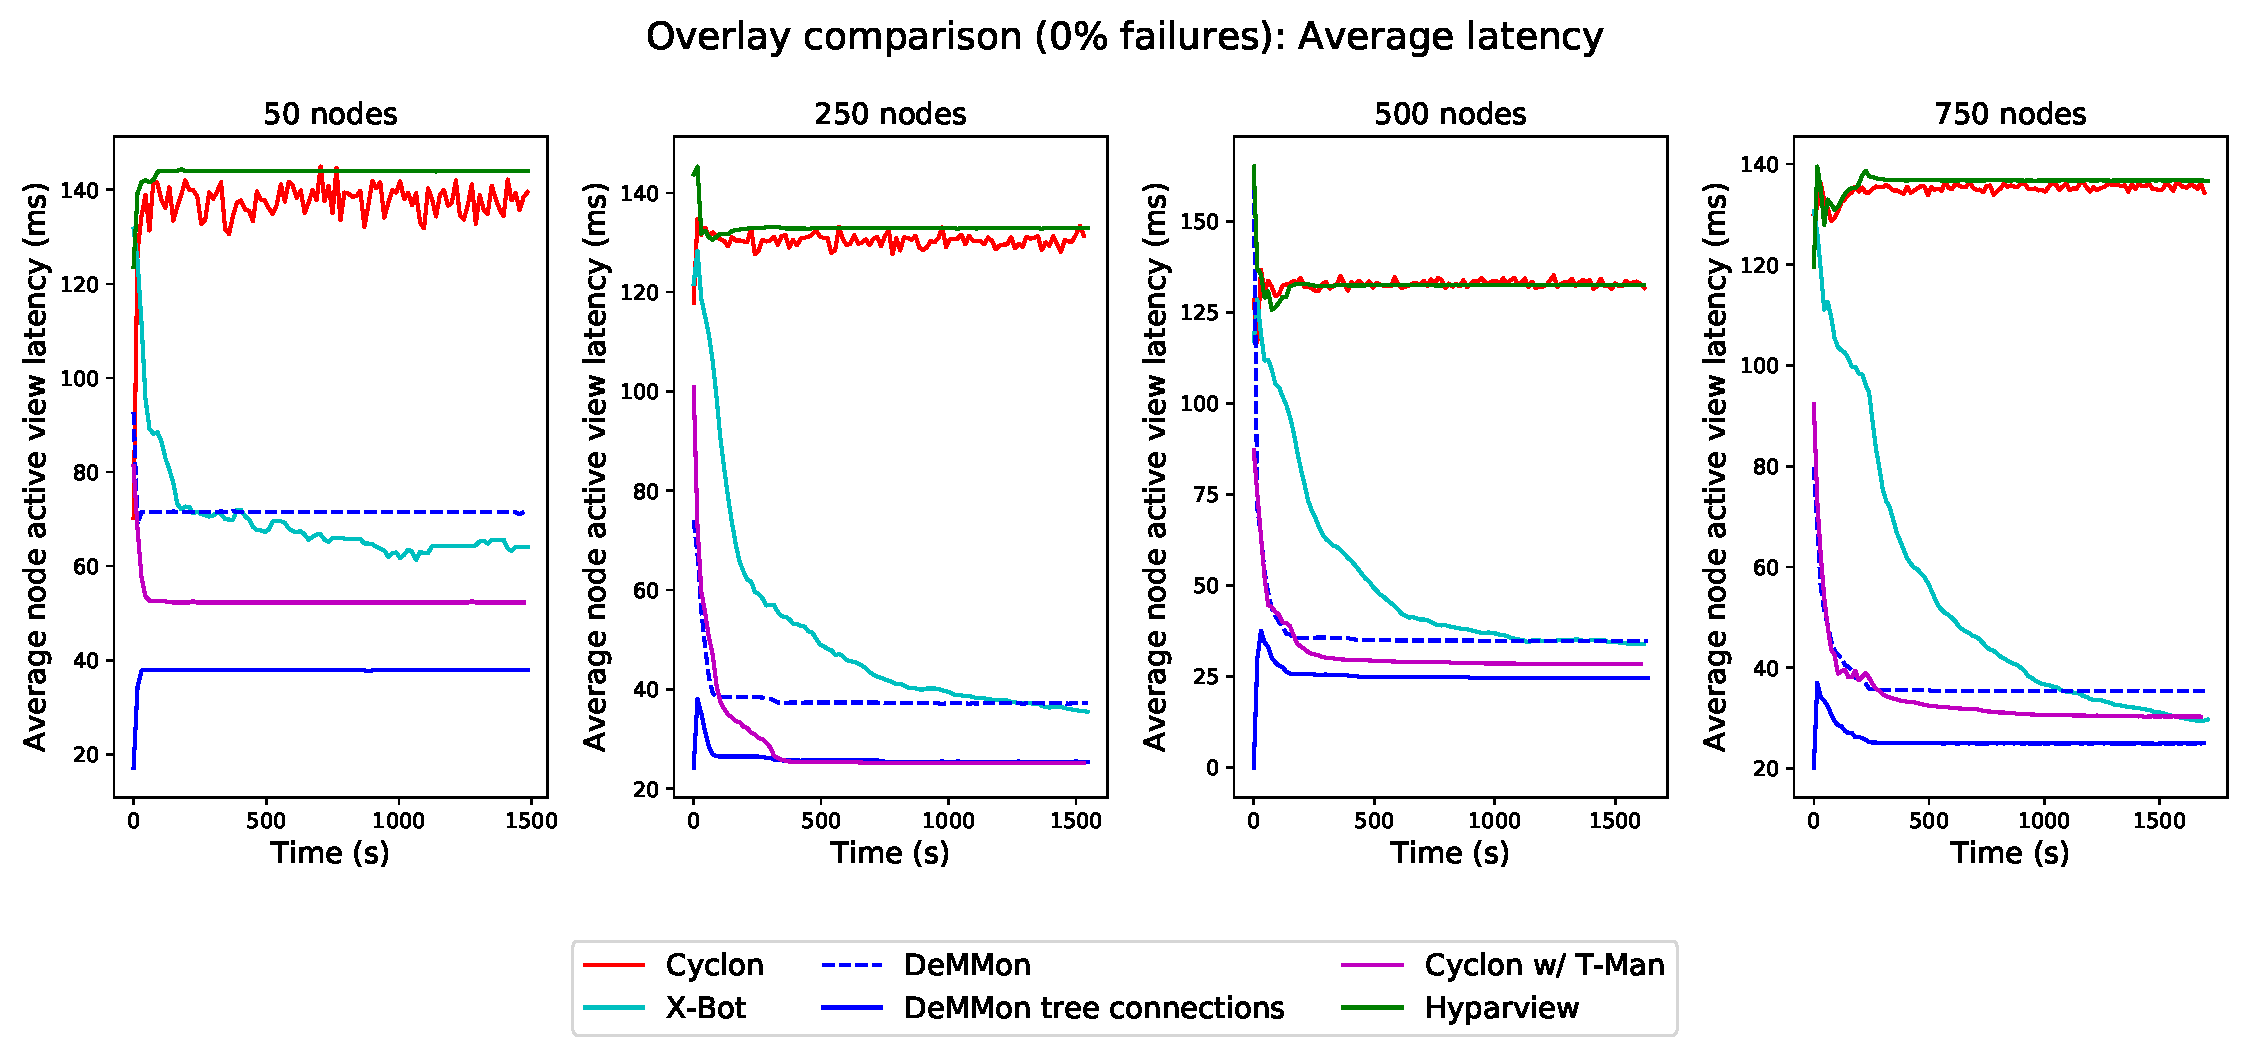
\includegraphics[width=\linewidth]{Chapters/evaluation/figures/membership/membership_lat_over_time_0_failures.pdf}
    \caption{Average latency in per node in established networks}
    \label{fig:overlay_proto_res_net_building:0_failures_lat}
\end{figure}


\begin{figure}
    \centering
    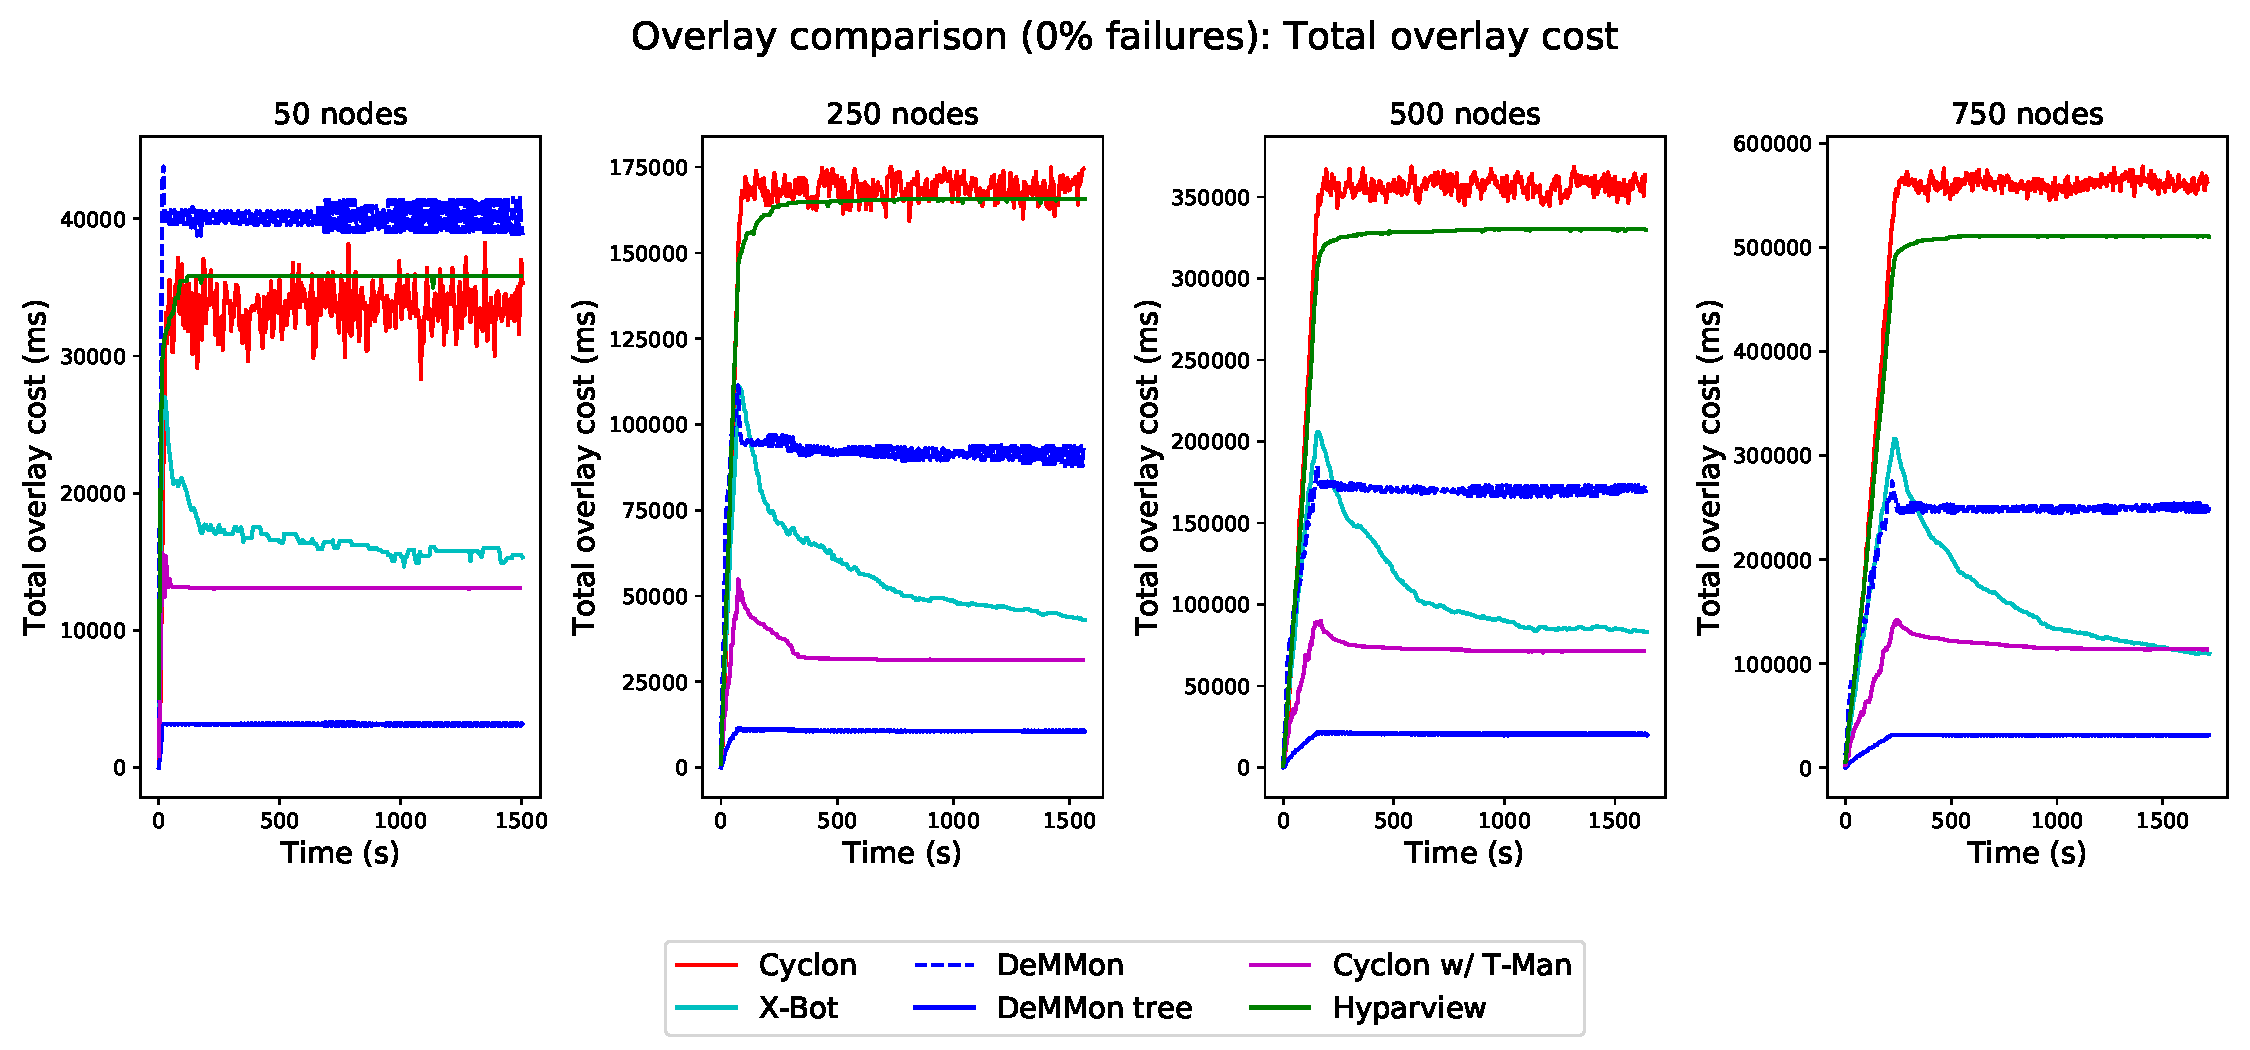
\includegraphics[width=\linewidth]{Chapters/evaluation/figures/membership/membership_total_lat_over_time_0_failures.pdf}
    \caption{Total network cost (in latency)}
    \label{fig:overlay_proto_res_net_building:0_failures_lat_total}
\end{figure}

In the figures \ref{fig:overlay_proto_res_net_building:0_failures_lat} and \ref{fig:overlay_proto_res_net_building:0_failures_lat_total}, we may observe the results pertaining to the average latency of a connection in the overlay and the total cost of the established overlay networks for an experiment with no failures. For both of these graphs, we show the results obtained from both the baseline protocols and the deMMon protocol. In the case of deMMon, we make a distinction between twos latency values, the first (represented by a blue continuous line) represents the results relative to all connections of all nodes, the second value (represented by a blue dashed line) represents the cost of the vertical connections of the deMMon tree (i.e. the parent and children of each node), essentially excluding the siblings of each node from the results. We made this distinction for two reasons: first, as the deMMon protocol only performs optimizations to improve the parent connection, we believe it is important to see the correllation from improving only the parent connections to the sibling latencies. The second reason to make this distinction is due to the fact that these connections are significantly more used when compared with the sibling connections for network maintenance, information dissemination and in-transit aggregation.

The results displayed in graphs \ref{fig:overlay_proto_res_net_building:0_failures_lat} and \ref{fig:overlay_proto_res_net_building:0_failures_lat_total} show that both hyparview and cyclon average their latencies at around the same values (which also correspond to the average of all connections of the latency matrix), which is expected as these protocols do not perform optimizations in regard to the network latency. The results also show that the devised protocol is the fastest in regard to converging to its lowest latency value, and that X-Bot is the slowest, not converging to a final value in a test of 25 minutes, which is expected as X-Bots' overlay improvements are performed using 7 messages, contrasting heavily with deMMons' 2 required messages, and T-Mans' 0 required messages for performing overlay improvements. While the total and average latency of the deMMon overlay is not the lowest in any of the displayed results, when comparing only the vertical connections, deMMon reaches a total latency cost lower than any other tested procotocol. This is important because as previously mentioned, these connections are the ones most used when performing overlay improvements and maintenance, information dissemination and in-transit aggregation. 

\begin{figure}
    \centering
    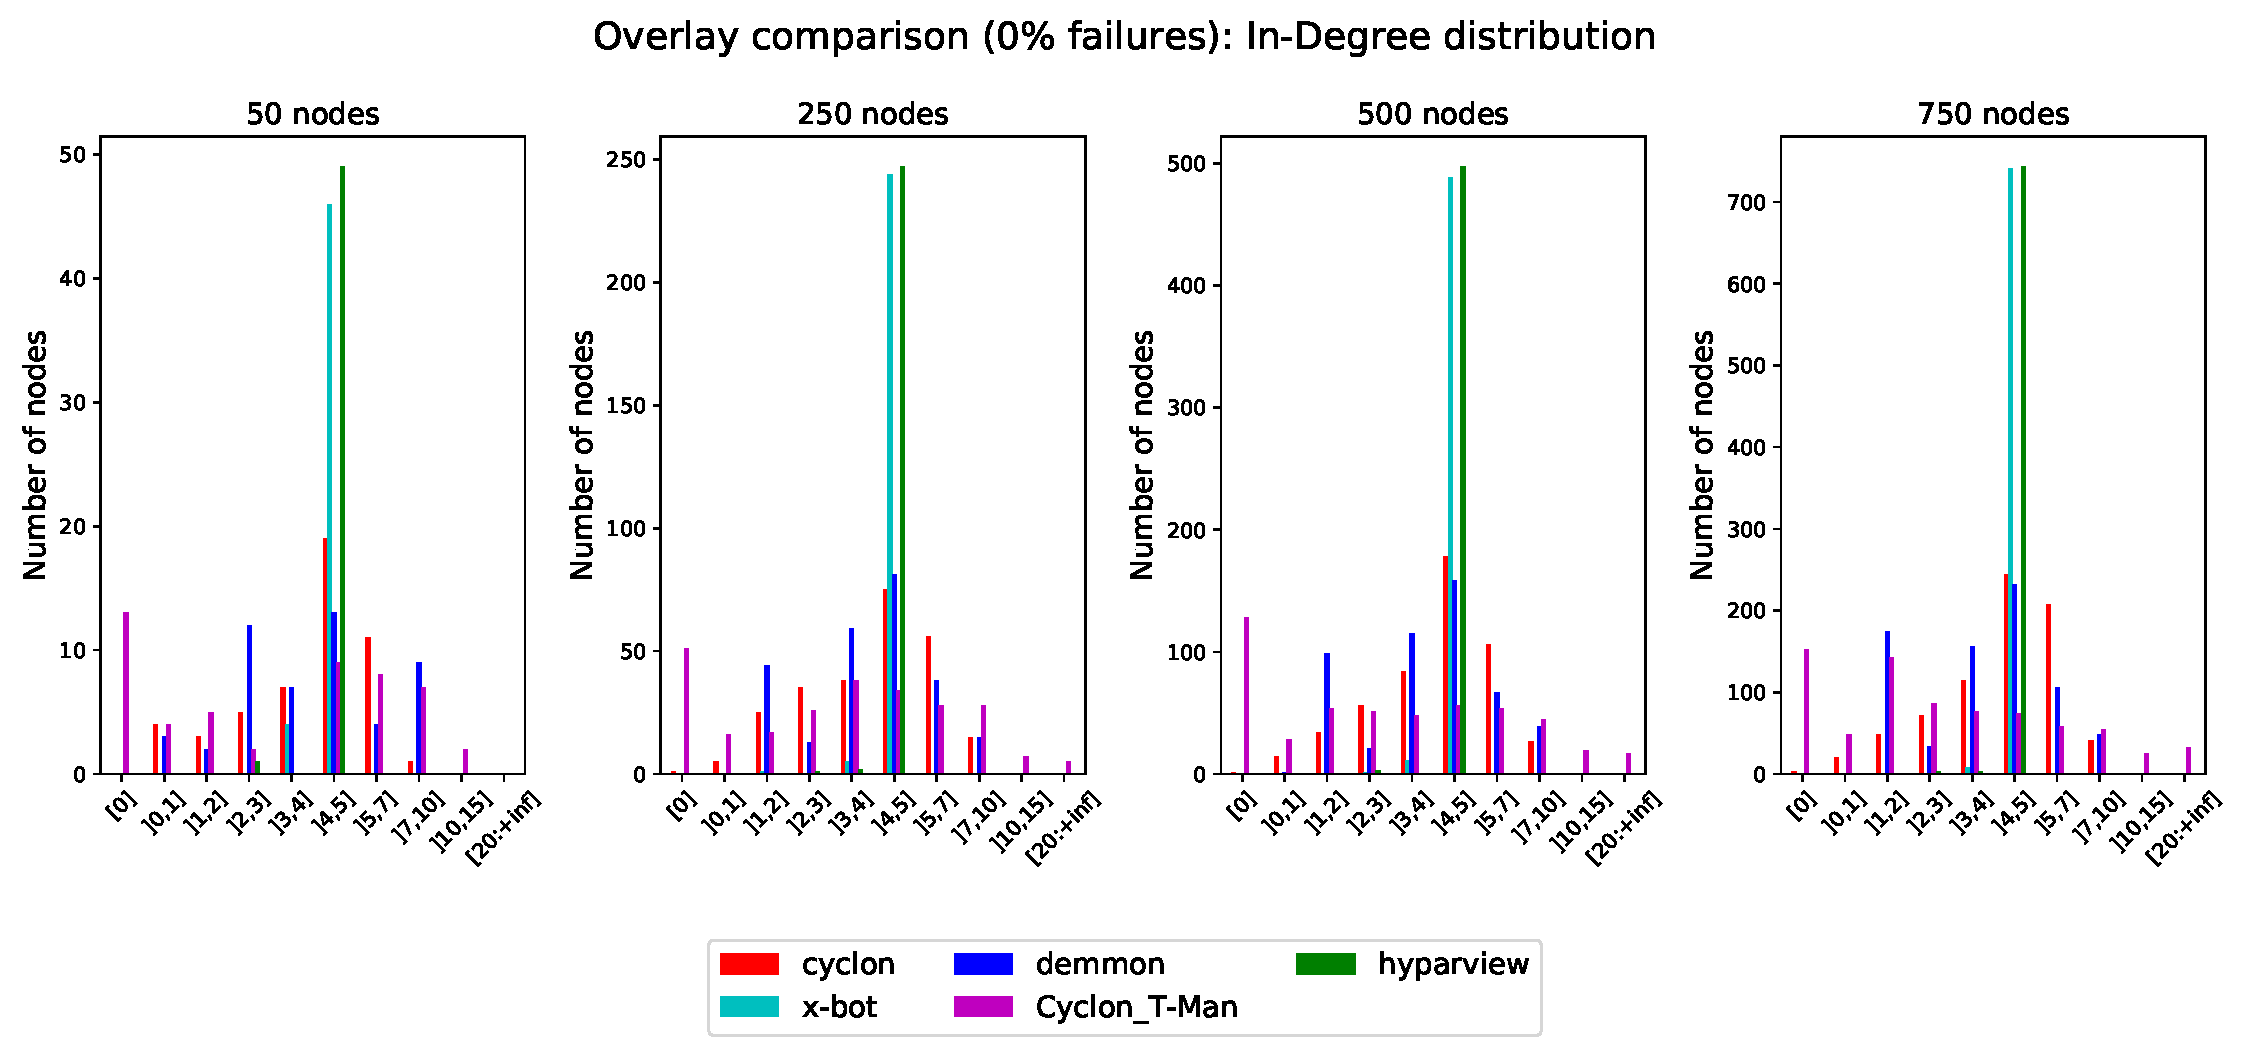
\includegraphics[width=\linewidth]{Chapters/evaluation/figures/membership/membership_inDegree_0_failures.pdf}
    \caption{Node in-degree}
    \label{fig:overlay_proto_res_net_building:0_failures_inDegree}
\end{figure}

It is important to mention that, while T-Man is the protocol that reaches the lowest overall and mean latency in the least amount of time, it does so disregarding the fact that nodes may become disconnected from overlay, which as we will observe further in this chapter, prevents this protocol from being a basis for reliable message dissemination. This factor may be observed in fig. \ref{fig:overlay_proto_res_net_building:0_failures_inDegree}, which shows the in-degree (the number of incoming connections for each node) for all nodes participating in the network for each tested protocol (these results correspond to the last configuration of the network before the experiment ended). These results show that T-Man, at multiple node counts, posesses nodes with 0 incoming connections, which are effectively isolated from the network. While still analyzing the in-degree results, we observe that both X-Bot and Hyparview have a fixed number of incoming connections, which results from the use of bidirectional connections, while cyclon has varied numbers of incoming connections ranging from 10 to 1, which occurs due to the shuffle mechanisms of the active connections. In the case of deMMon, the values range from 2 to 10 incoming connections, which is expected given the configuration parameters of a minimum number of children of 2, and a maximum number of children of 5 (which as previously mentioned, is not guaranteed to bound the number of children).


\begin{figure}
    \centering
    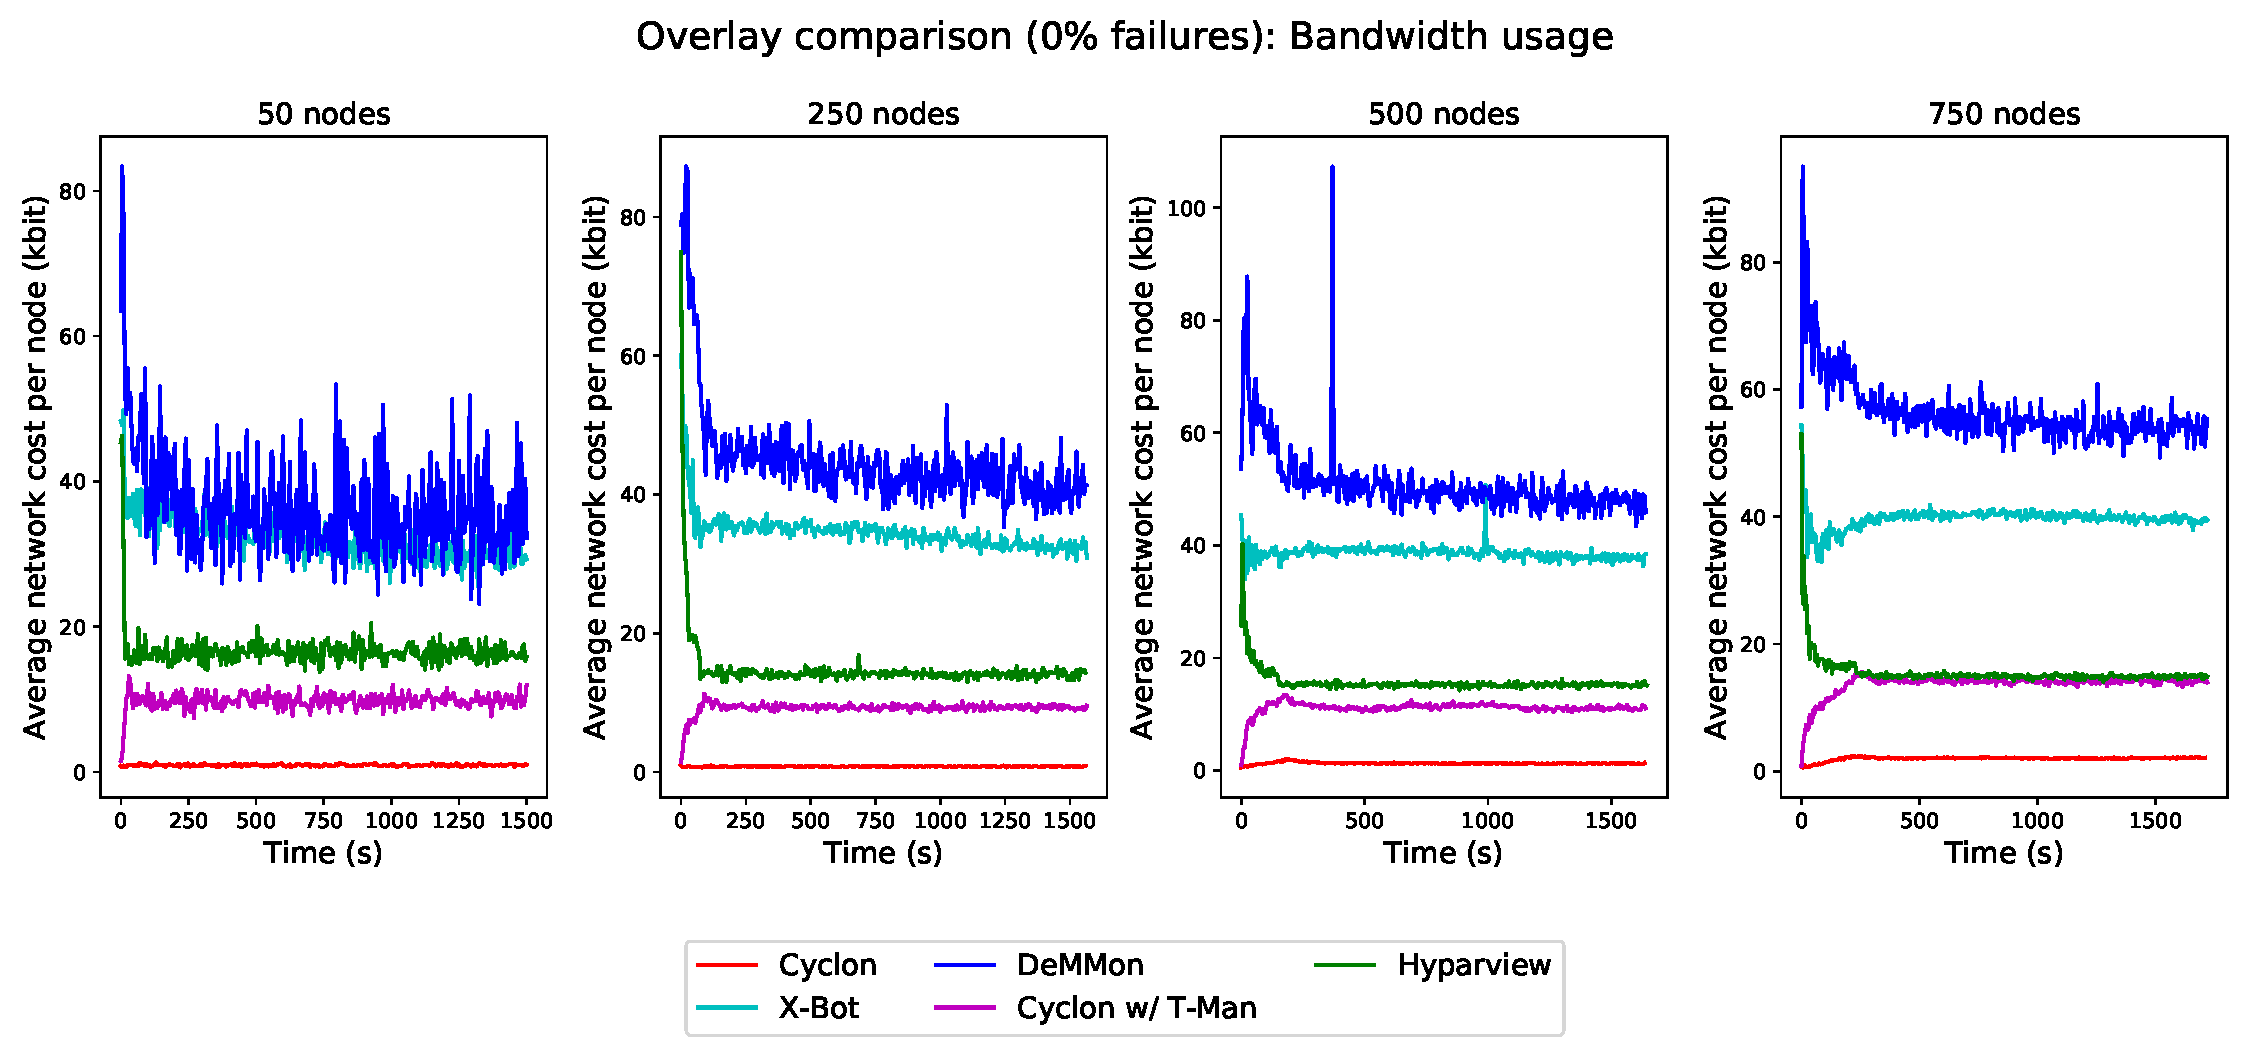
\includegraphics[width=\linewidth]{Chapters/evaluation/figures/membership/membership_bw_over_time_0_failures.pdf}
    \caption{Protocol bandwidth cost}
    \label{fig:overlay_proto_res_net_building:0_failures_BWUsage}
\end{figure}

Finally, still regarding the experiments without node failures, we show in figure \ref{fig:overlay_proto_res_net_building:0_failures_BWUsage} the average network cost (in kbit/5s) incurred by each node running the experiments. This graph shows that deMMons' overlay protocol, on average, spends more bandwidth to build and maintain the network structure, we believe this is due to the fact that deMMon exchanges more information periodically with peers in the active view (to maintain an improve the tree structure) when compared to the other protocols. Conversely, the protocol which uses the least amount of bandwidth is Cyclon, as its shuffle mechanism is relatively inexpensive and the protocol posesses no other mechanisms. Although protocols have varied networking costs, we believe that even deMMon which uses more bandwidth is relatively inexpensive when compared with the bandwidth standards at the time of writing this work.

\begin{figure}
    \centering
    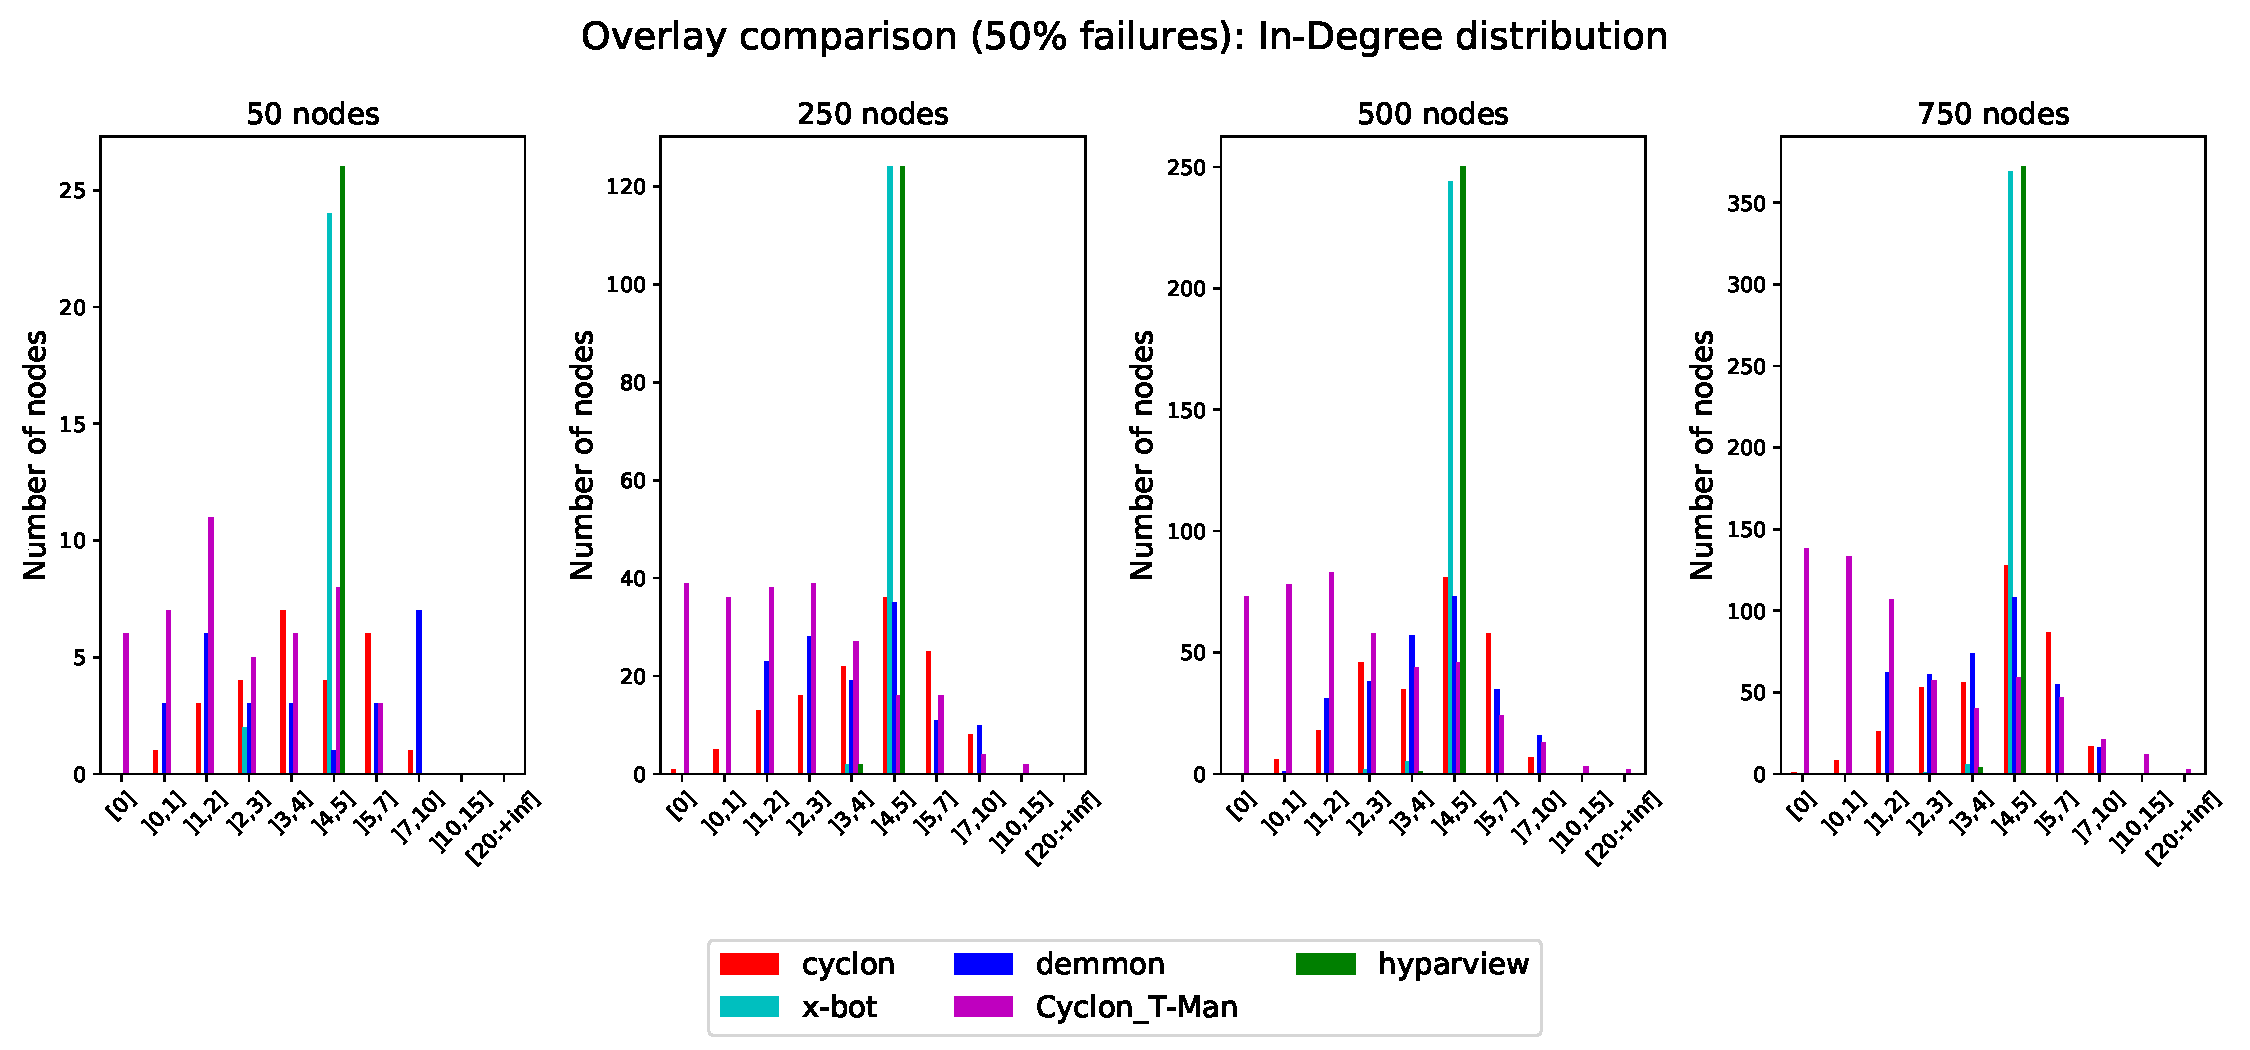
\includegraphics[width=\linewidth]{Chapters/evaluation/figures/membership/membership_inDegree_50_failures.pdf}
    \caption{Node in-degree (50\% failures)}
    \label{fig:overlay_proto_res_net_building:50_failures_inDegree}
\end{figure}

Provided with the result analysis for the experiments with no failures, we now provide the results for the in-degree distribution of the protocol in a scenario with failures. This second experiment tests the fault tolerance of the protocols by first establishing the network (similarly to the first scenario), however, during the middle of the experiment, we induce a catastrophic failure of 50\% of the nodes. The objective of this experiment was to test if any node became isolated from the network after this period of failures. Results from this experiment may be observed in figure \ref{fig:overlay_proto_res_net_building:50_failures_inDegree}, where it is observable that, for all tested protocols except T-Man, no nodes became isolated, allowing us to conclude that the devised protocol can recover from faults effectively.

As previously mentioned, the aplicability of our solution was tested in two different aspects: the first was the process of building and maintaining the overlay network, which was covered the previous paragraphs. The second evaluated aspect is information dissemination (via message broadcasting), which we will now cover in the following subsection.

\todo{meter resultados grandes em anexo?}

\subsection{Information dissemination}

The second set of conducted experiments, as mentioned previously, intends to test the applicability of the devised membership protocol in an information dissemination scenario. To do so, we tested it against the same set of baseline protocols used in the previous experiments enriched with two message dissemination protocols: the first is a simple flood protocol, where if a node wishes to broadcast a message, it sends that message to every peer in its active view, then, nodes that receive this message, propagate it to every neighbour if they havent done so previously (excluding the sender). The second used dissemination protocol was PlumTree \todo{cite}, which is a dissemination protocol that builds a dissemination tree rooted on the first node that issues a broadcast message. The reasoning behind this choice of dissemination protocols was to provide a fairer comparison of deMMon with the remaining protocols, as we believe that because simple flood generates many redundant messages when compared to dissemination using only a tree structure, it would be unfair to not include a dissemination protocol which also employs a tree, similarly to deMMon. It is important to mention that, when testing the PlumTree protocol,in order to establish the initial tree, in the experiments for this protocol a single node first establishes the tree by starting the dissemination of its messages a minute earlier. For both of these comparisons, deMMon is set up with a dissemination protocol similar to the simple flood protocol, however only using its vertical connections (parent and children).

Similarly to the first set of experiments, we conducted multiple tests with 50, 250, 500 and 750 nodes during 15 minute periods, for all these node numbers we also tested failure rates of 0 and 50\% of the system. For each of these node numbers and failure rates, we varied the number of messages each node emitted until all protocols reach their saturation point. While doing the tests, we extracted the following metrics: (1) the reliability of the messages, i.e. what is the percentage of nodes participating in the overlay at the time of emission of a certain message that receive that message; (2) the maximum message throughput reached by every protocol in a 30 second window, (3) the average latency taken by messages until they reach their destination, and (4) the bandwidth usage of each of the protocols. 

\begin{figure}[htbp]
    \centering
    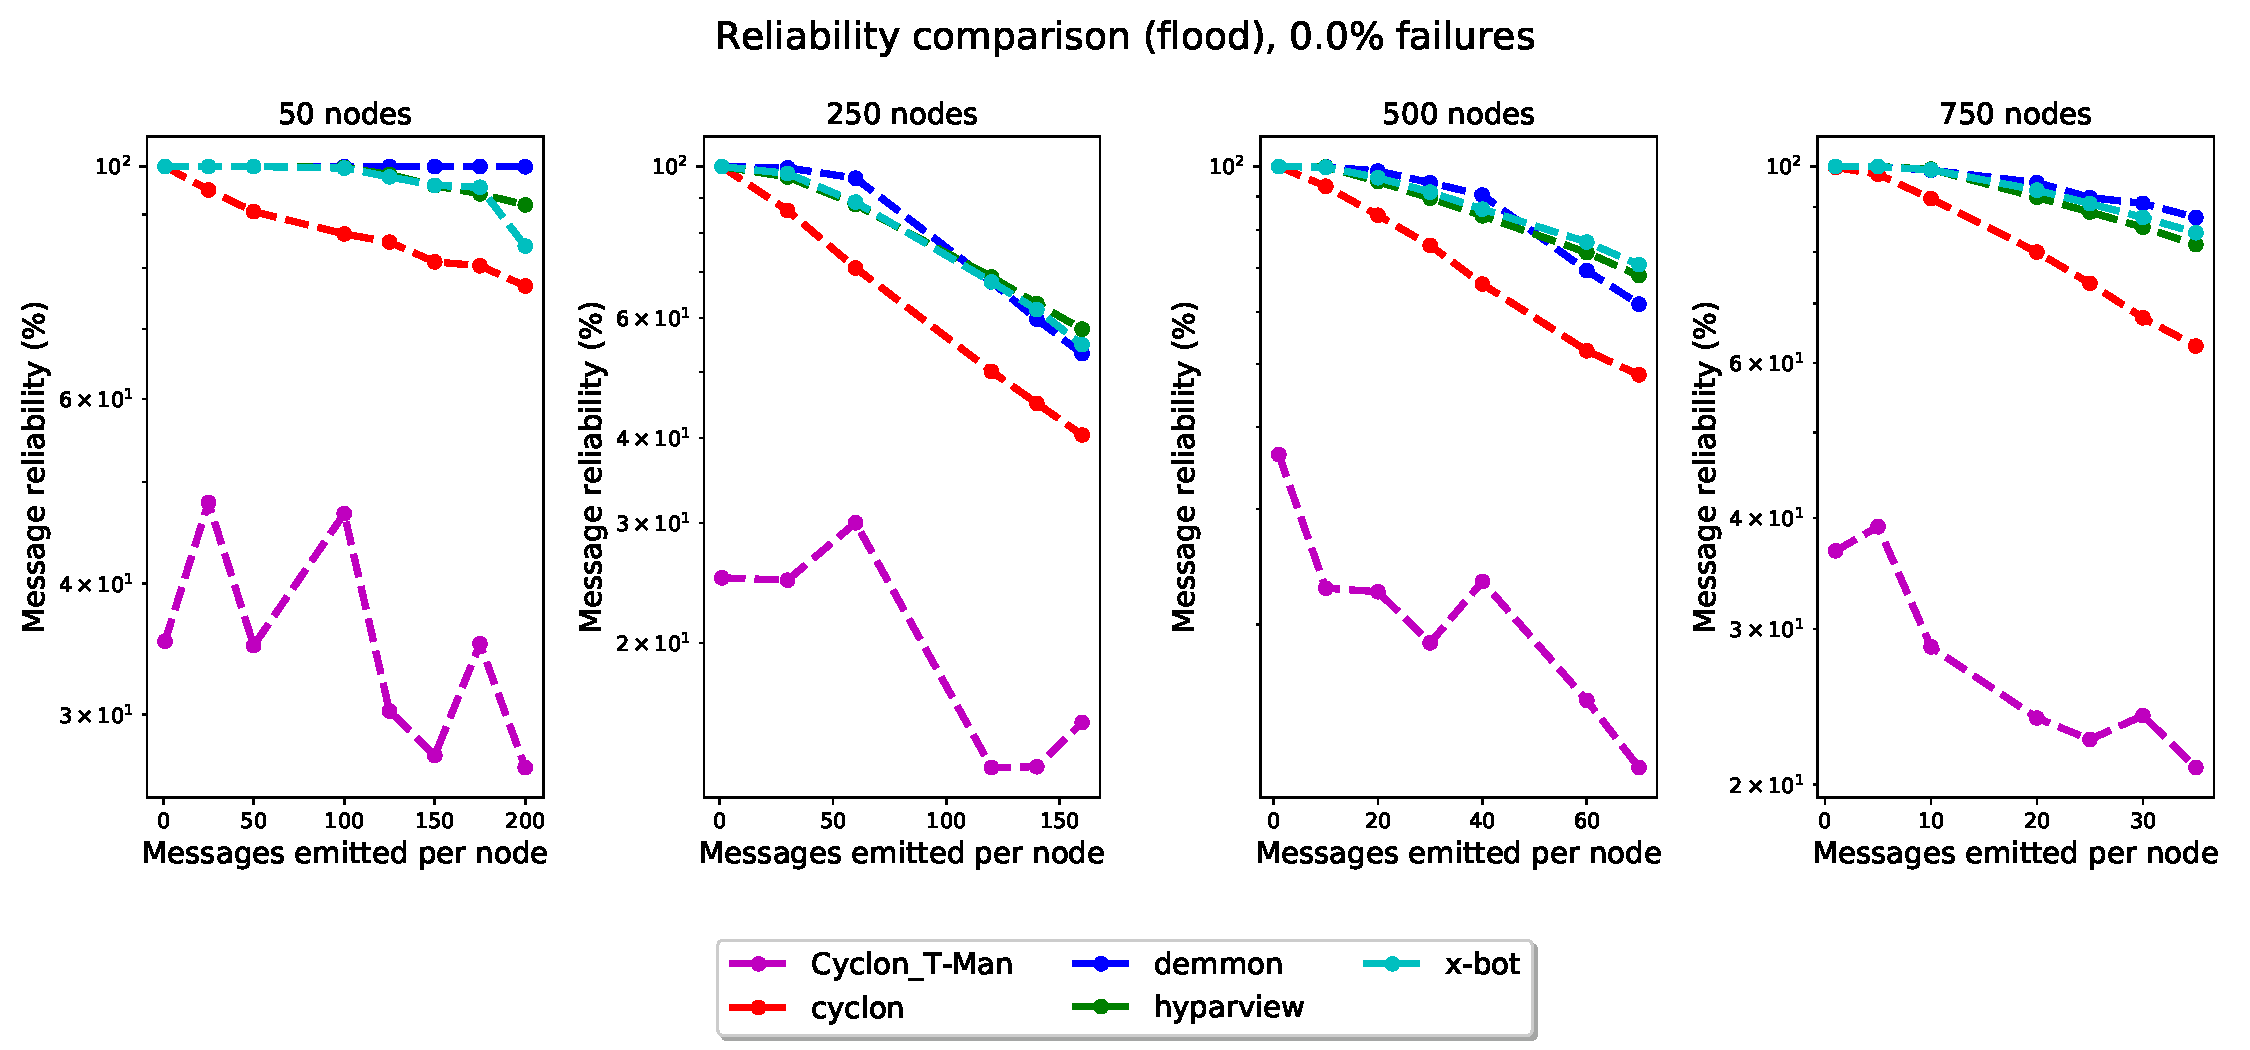
\includegraphics[width=\linewidth]{Chapters/evaluation/figures/flood/flood_0.0_failures_reliability.pdf}
    \caption{Average message reliability in simple flood scenario (0\% failures)}
    \label{fig:overlay_proto_res_msg_diss:0_failures_reliability_flood}
\end{figure}

\begin{figure}[htbp]
    \centering
    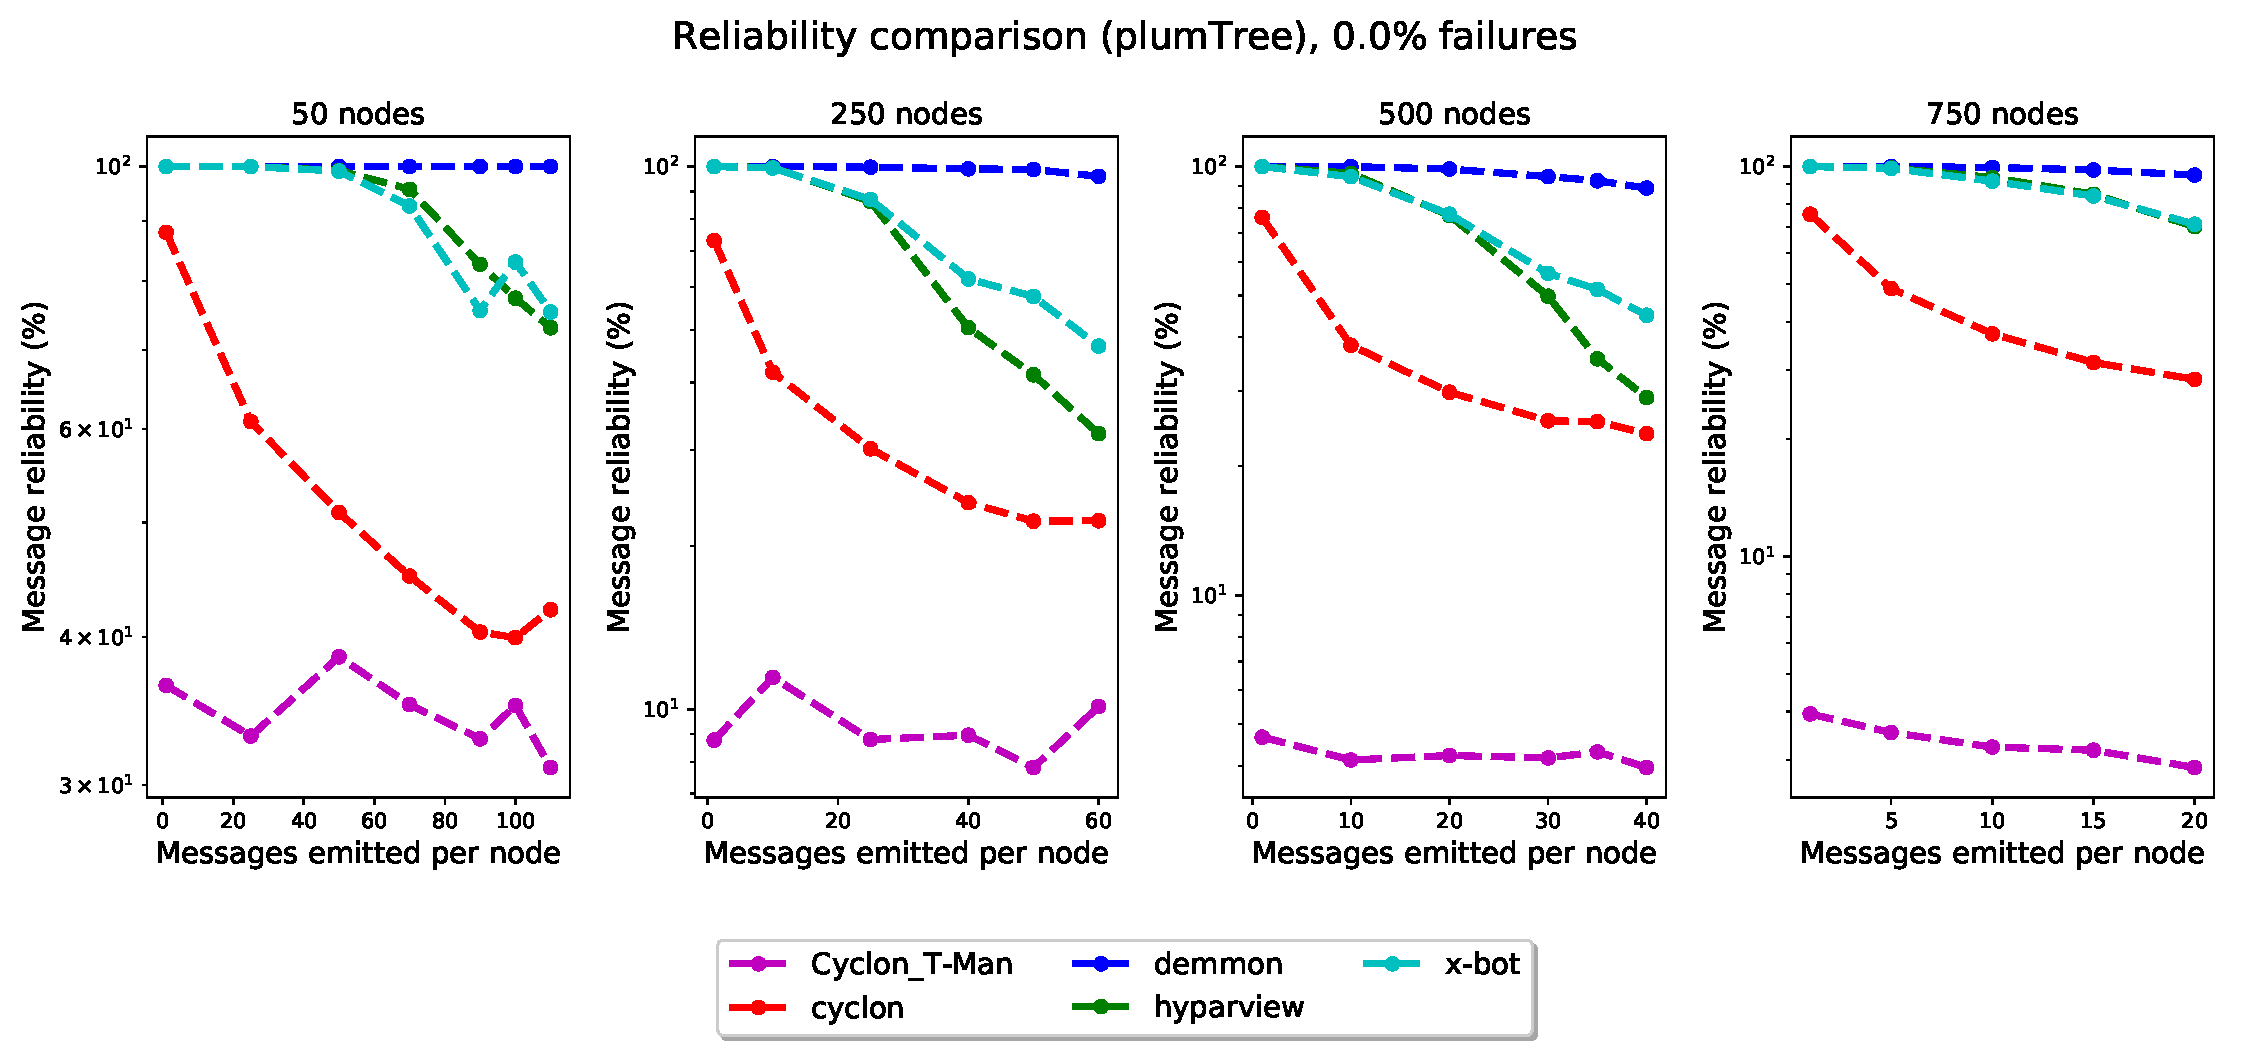
\includegraphics[width=\linewidth]{Chapters/evaluation/figures/flood/plumTree_0.0_failures_reliability.pdf}
    \caption{Average message reliability in PlumTree scenario (0\% failures)}
    \label{fig:overlay_proto_res_msg_diss:0_failures_reliability_plumTree}
\end{figure}

Figures \ref{fig:overlay_proto_res_msg_diss:0_failures_reliability_flood} and \ref{fig:overlay_proto_res_msg_diss:0_failures_reliability_plumTree} show the obtained results regarding the message reliability during the experiments for both the simple flood and plumTree experiments with 0 failures. As we may observe, in general, the saturation point for all protocols using PlumTree tends to be earlier (in terms of emitted messages per node) than the simple flood protocol. We believe this occurs because the PlumTree protocols' tree becomes unstable whenever certain nodes become a bottleneck to the messages being propagated using the tree because their bandwidth is exceeded. Whenever this occurs, as certain messages are delayed, the tree structure becomes unstable (as the order of delivery of messages is what defines the dissemination tree structure). Whenever this occurs, the tree repair procedure is triggered, however, as there are multiple nodes emitting new messages simultaneously, and new nodes can become saturated while performing this mechanism, the tree structure may never reconverge until all messages are delivered. Until this occurs, the protocol essentially becomes a push-pull gossip protocol, which has lower performance in our experiments in terms of reliability, because the tests end before the protocol has delivered all messages.

In addition to the previously mentioned reasons, in an ocasions where a node has received an IHAVE message for a certain message ID, and happens to have available upload bandwidth but its download capacity is all taken up by incomming traffic, this node will periodically emit GRAFT messages to the sender of the IHAVE nessage, which will reply with broadcast messages that are only received after a large time frame. Whenever this occurs, there are multiple redundant GRAFT and IHAVE messages being emitted, which results in the system possibly becoming even more saturated, which causes the tree to become even more unstable. The devised overlay protocol, although it also uses a tree structure, given that the tree is not defined by the propagations of broadcast messages, it is not as susceptible to instability in conditions where the network is saturated, consequently achieving higher reliability in higher message counts. 

We may observe that both the Cyclon and T-Man tend to perform worse in general regard to reliability when compared to deMMon, Hyparview and DeMMon, which we believe, in the case of T-Man, to occur because there are nodes with 0 incomming connections which do not receive any broadcast messages from other nodes, and in the case of cyclon we believe the drop in reliability is attributed to the use of UDP as a its communication medium, which means that whenever the data channels becomes saturated, many of the broadcast messages are lost, contrary to deMMon, hyparview and X-BOT, that use TCP and do not drop messages in congestion periods. Finally, we believe that both cyclon and T-MAN when paired with plumTree have particularly lower reliability for because this protocol requires bidirectional connections to perform optimally, which are not guaranteed in either of these protocols. 

In regard to the simple flood experiment (fig. \ref{fig:overlay_proto_res_msg_diss:0_failures_reliability_flood}), deMMon tends to perform exceptionally well with fewer node counts, particularly with 50 nodes, we believe this may be due to the height of the deMMon tree being smaller, as when the tree heigh is smaller, the number of descendants for each node is fewer, which in turn means that when a certain node becomes saturated, fewer nodes are impacted by this. In higher node counts, deMMon performs in line with both Hyparview and X-Bot. We believe this happens because the tradeoffs of having a tree (a single node possibly becoming a bottleneck for many other nodes in the system) tend to impact the system the same amount that sending multiple redundant messages does. 

\begin{figure}[htbp]
    \centering
    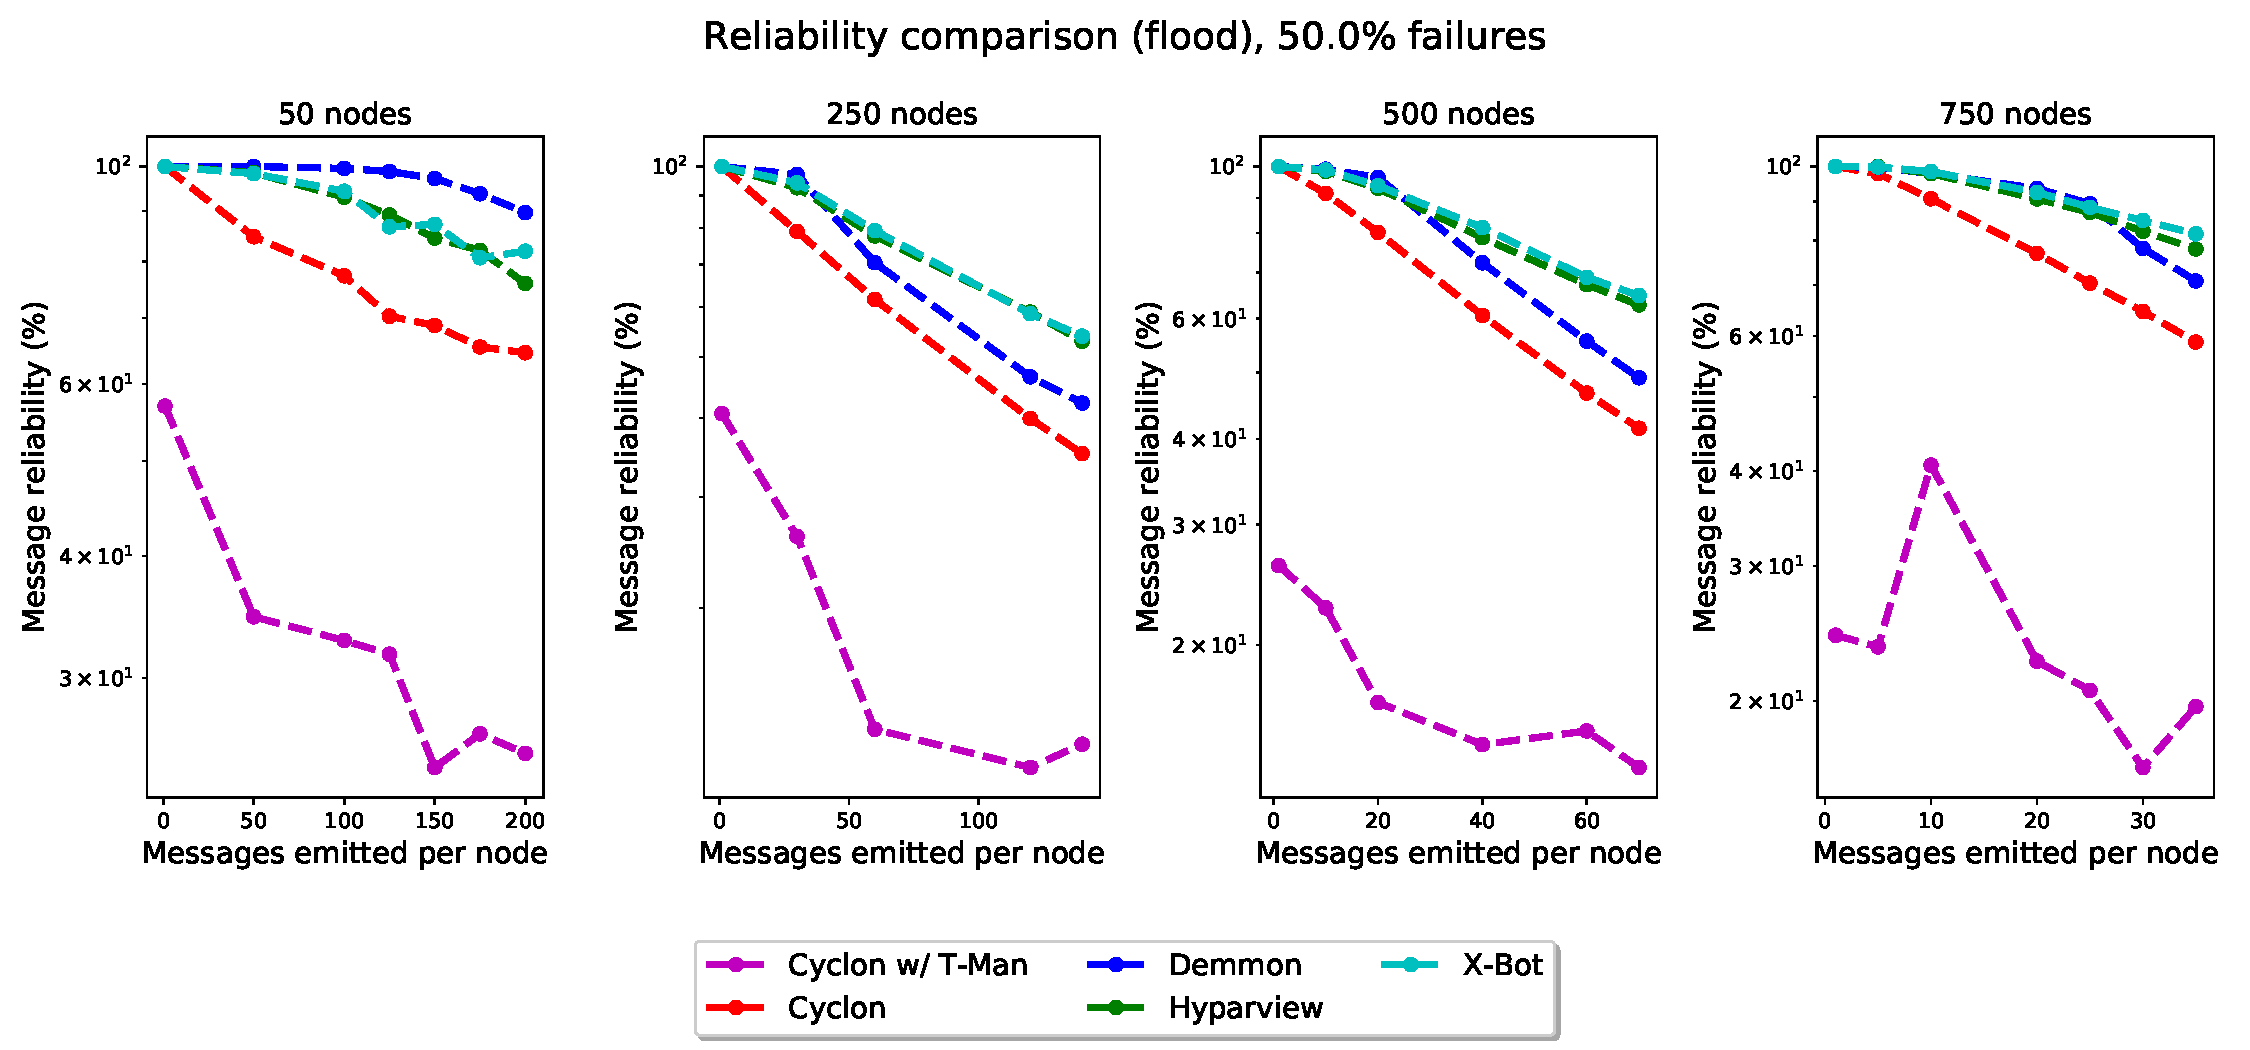
\includegraphics[width=\linewidth]{Chapters/evaluation/figures/flood/flood_50.0_failures_reliability.pdf}
    \caption{Average message reliability in simple flood scenario (50\% failures)}
    \label{fig:overlay_proto_res_msg_diss:50_failures_reliability_flood}
\end{figure}

\begin{figure}[htbp]
    \centering
    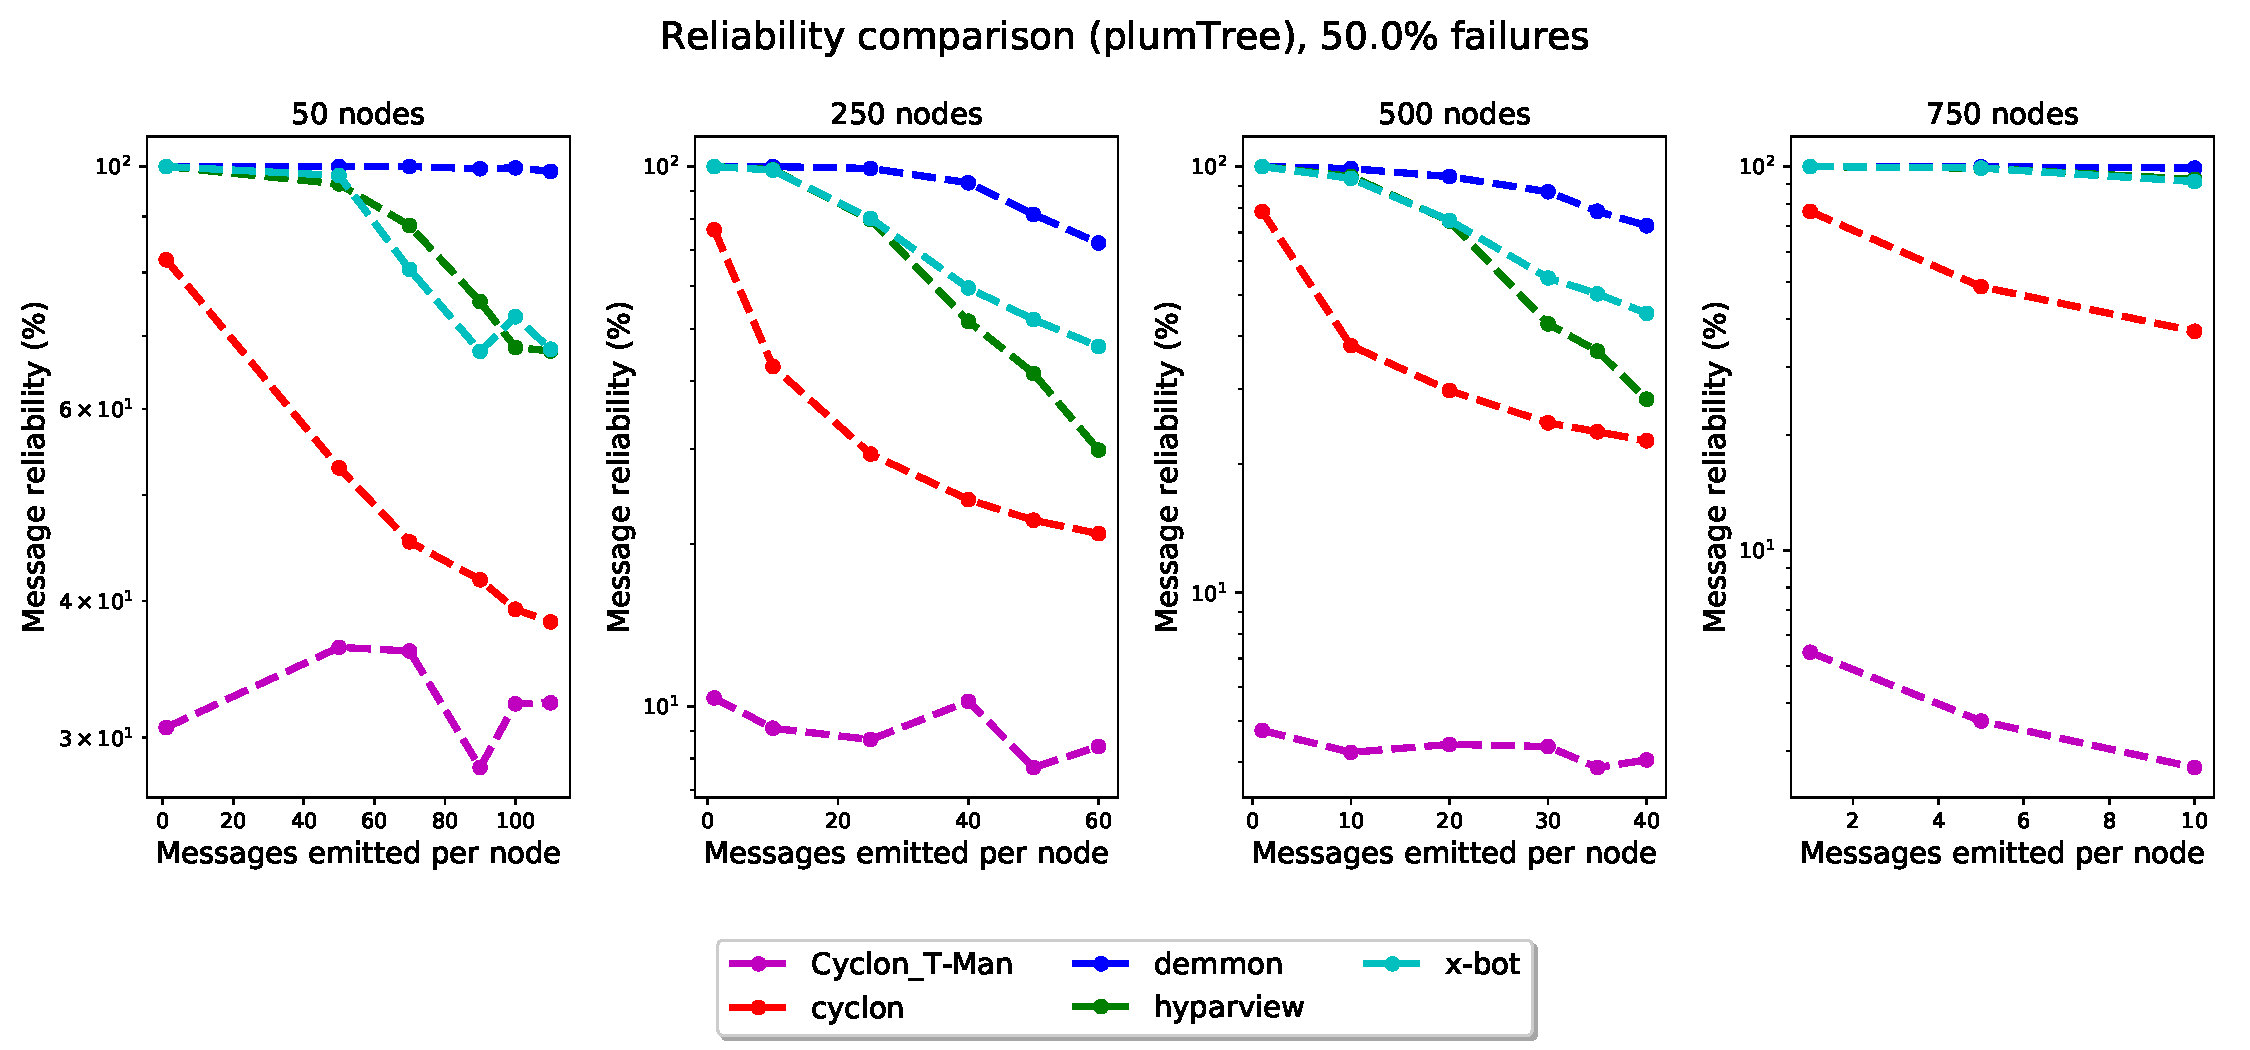
\includegraphics[width=\linewidth]{Chapters/evaluation/figures/flood/plumTree_50.0_failures_reliability.pdf}
    \caption{Average message reliability in PlumTree scenario (50\% failures)}
    \label{fig:overlay_proto_res_msg_diss:50_failures_reliability_plumTree}
\end{figure}

In the case of scenarios with induced failures (figures \ref{fig:overlay_proto_res_msg_diss:50_failures_reliability_flood} and \ref{fig:overlay_proto_res_msg_diss:50_failures_reliability_plumTree}), we observe a similar trend in regard to the plumTree experiments, with deMMon achieving higher reliability values. However, in the simple flood experiments, we observe that deMMon achieves a lower reliability value when under congestion, we believe this occurs because as the failures are occurring, if the nodes are saturated and lose their parent, the failure recovery mechanisms may take a long time frame to execute, and during this period nodes are disconnected from the remaining overlay and consequently do not receive or send message to any node which is not their descendant, leading to a lower reliability value.

Provided the results from the combination of the baseline protocols with PlumTree consistently performs worse in terms of reliability (when the network is saturated) when compared to employing only a simple flood protocol, we now focus on the comparison between deMMon and the baseline protocols executing the simple flood protocol, however, all obtained results are available in annex \todo{put the results in annex, and ref}.

\begin{figure}[htbp]
    \centering
    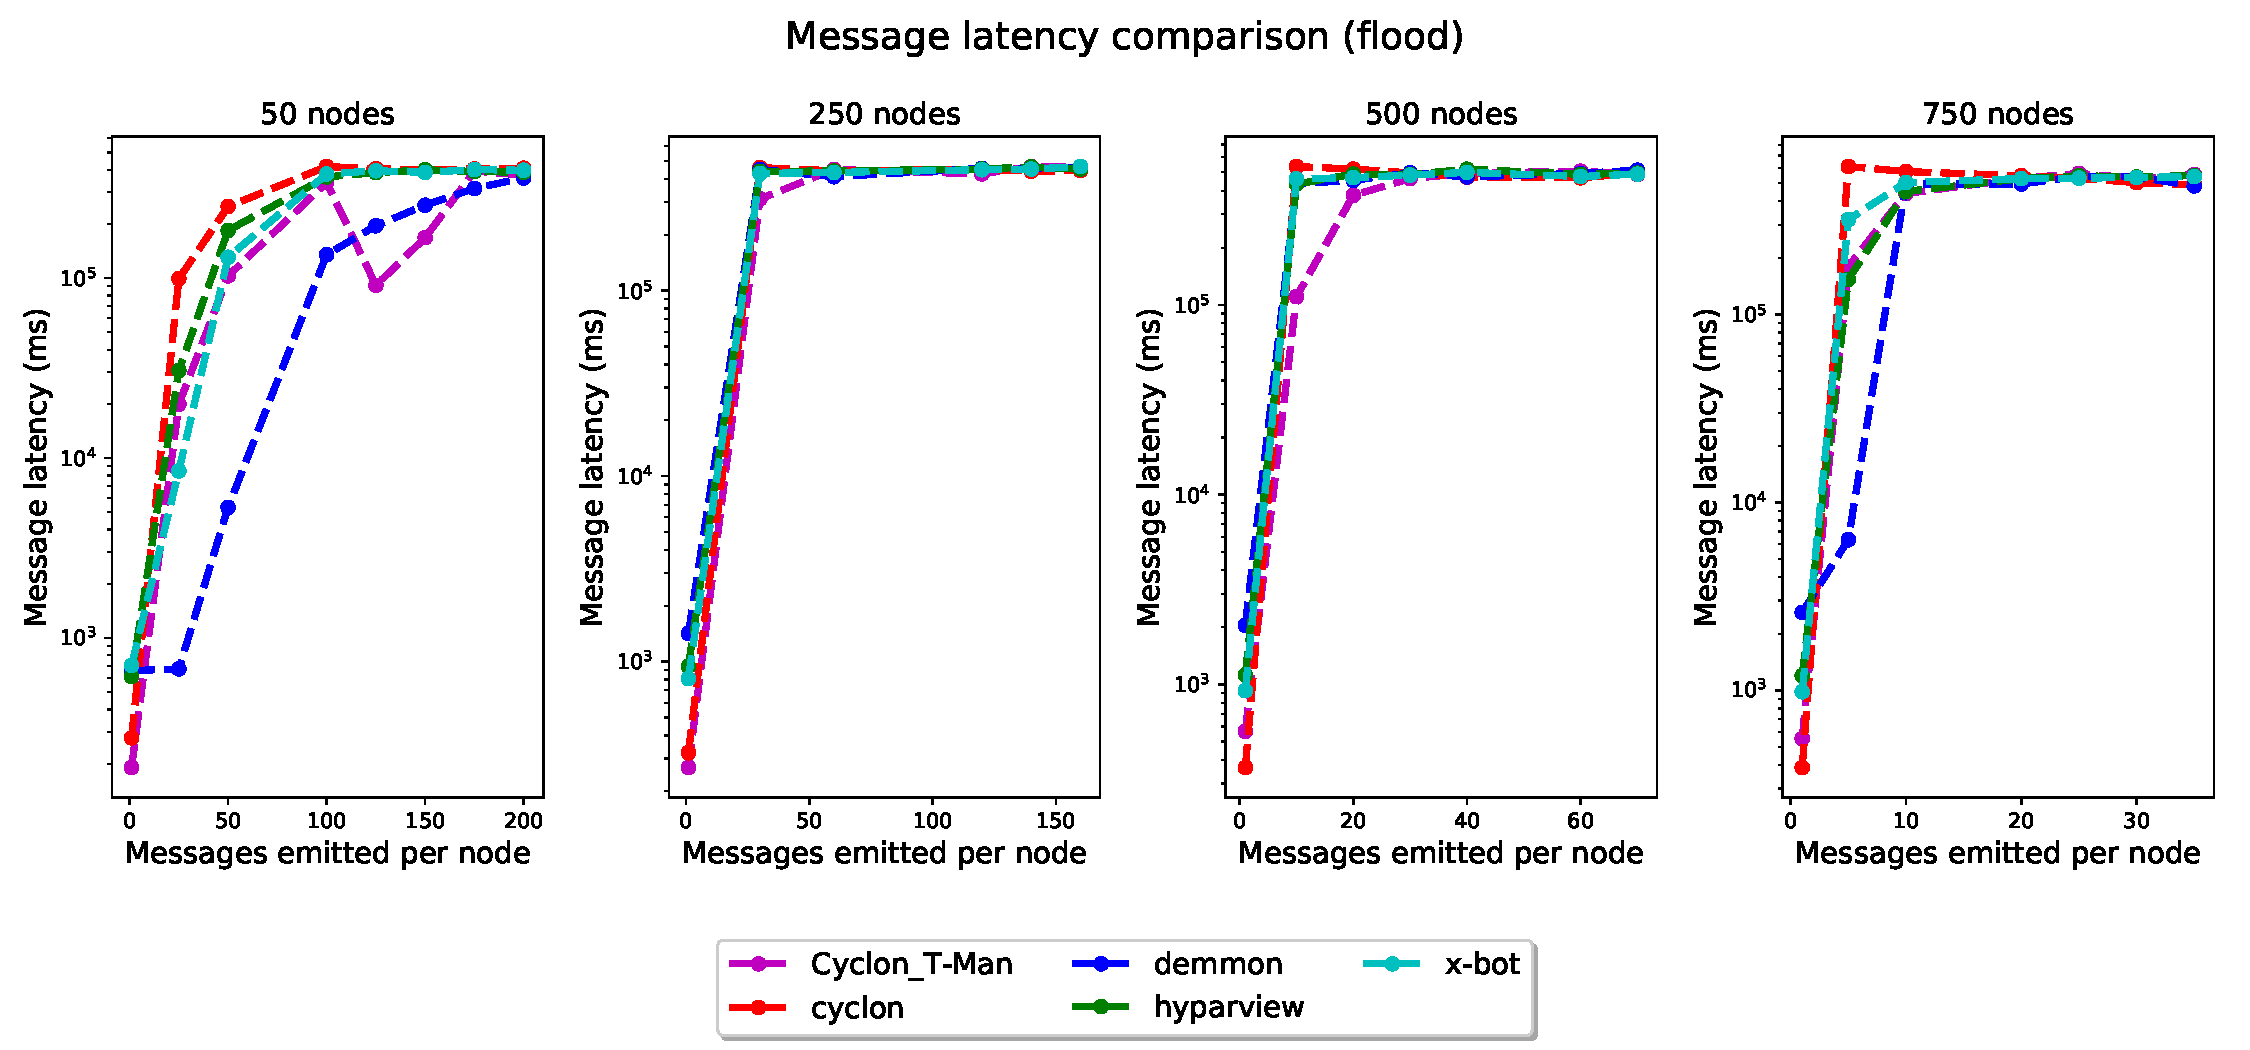
\includegraphics[width=\linewidth]{Chapters/evaluation/figures/flood/flood_0.0_failures_msg_lat.pdf}
    \caption{Average message latency (in ms) in simple flood scenario (0\% failures)}
    \label{fig:overlay_proto_res_msg_diss:0_failures_latency_flood}
\end{figure}

In figure \ref{fig:overlay_proto_res_msg_diss:0_failures_latency_flood} we may observe the obtained results from collecting the latency between the emition and reception of the message for each node. The first takeaway from these results is that all protocols plateau at the same latency value, this is due to the fact the the test times are limited to 15 minutes, and whenever the system is saturated, all messages tend to take a similarly long time to be delivered, and those which are not delivered are only reflected in the previously discussed reliability graphs (figures \ref{fig:overlay_proto_res_msg_diss:0_failures_reliability_flood}, \ref{fig:overlay_proto_res_msg_diss:0_failures_reliability_plumTree}, \ref{fig:overlay_proto_res_msg_diss:50_failures_reliability_flood}, and \ref{fig:overlay_proto_res_msg_diss:50_failures_reliability_plumTree}). However, for lower message counts, the latency results show that deMMon tends to achieve lower latency values when compared with the baseline protocols on certain workloads (e.g. low numbers of messages emitted on both the 50 and 750 node graphs) where we believe the flood protocol becomes saturated due to the number of redundant messages sent, whereas deMMon must send less messages to perform the message dissemination.

\begin{figure}[htbp]
    \centering
    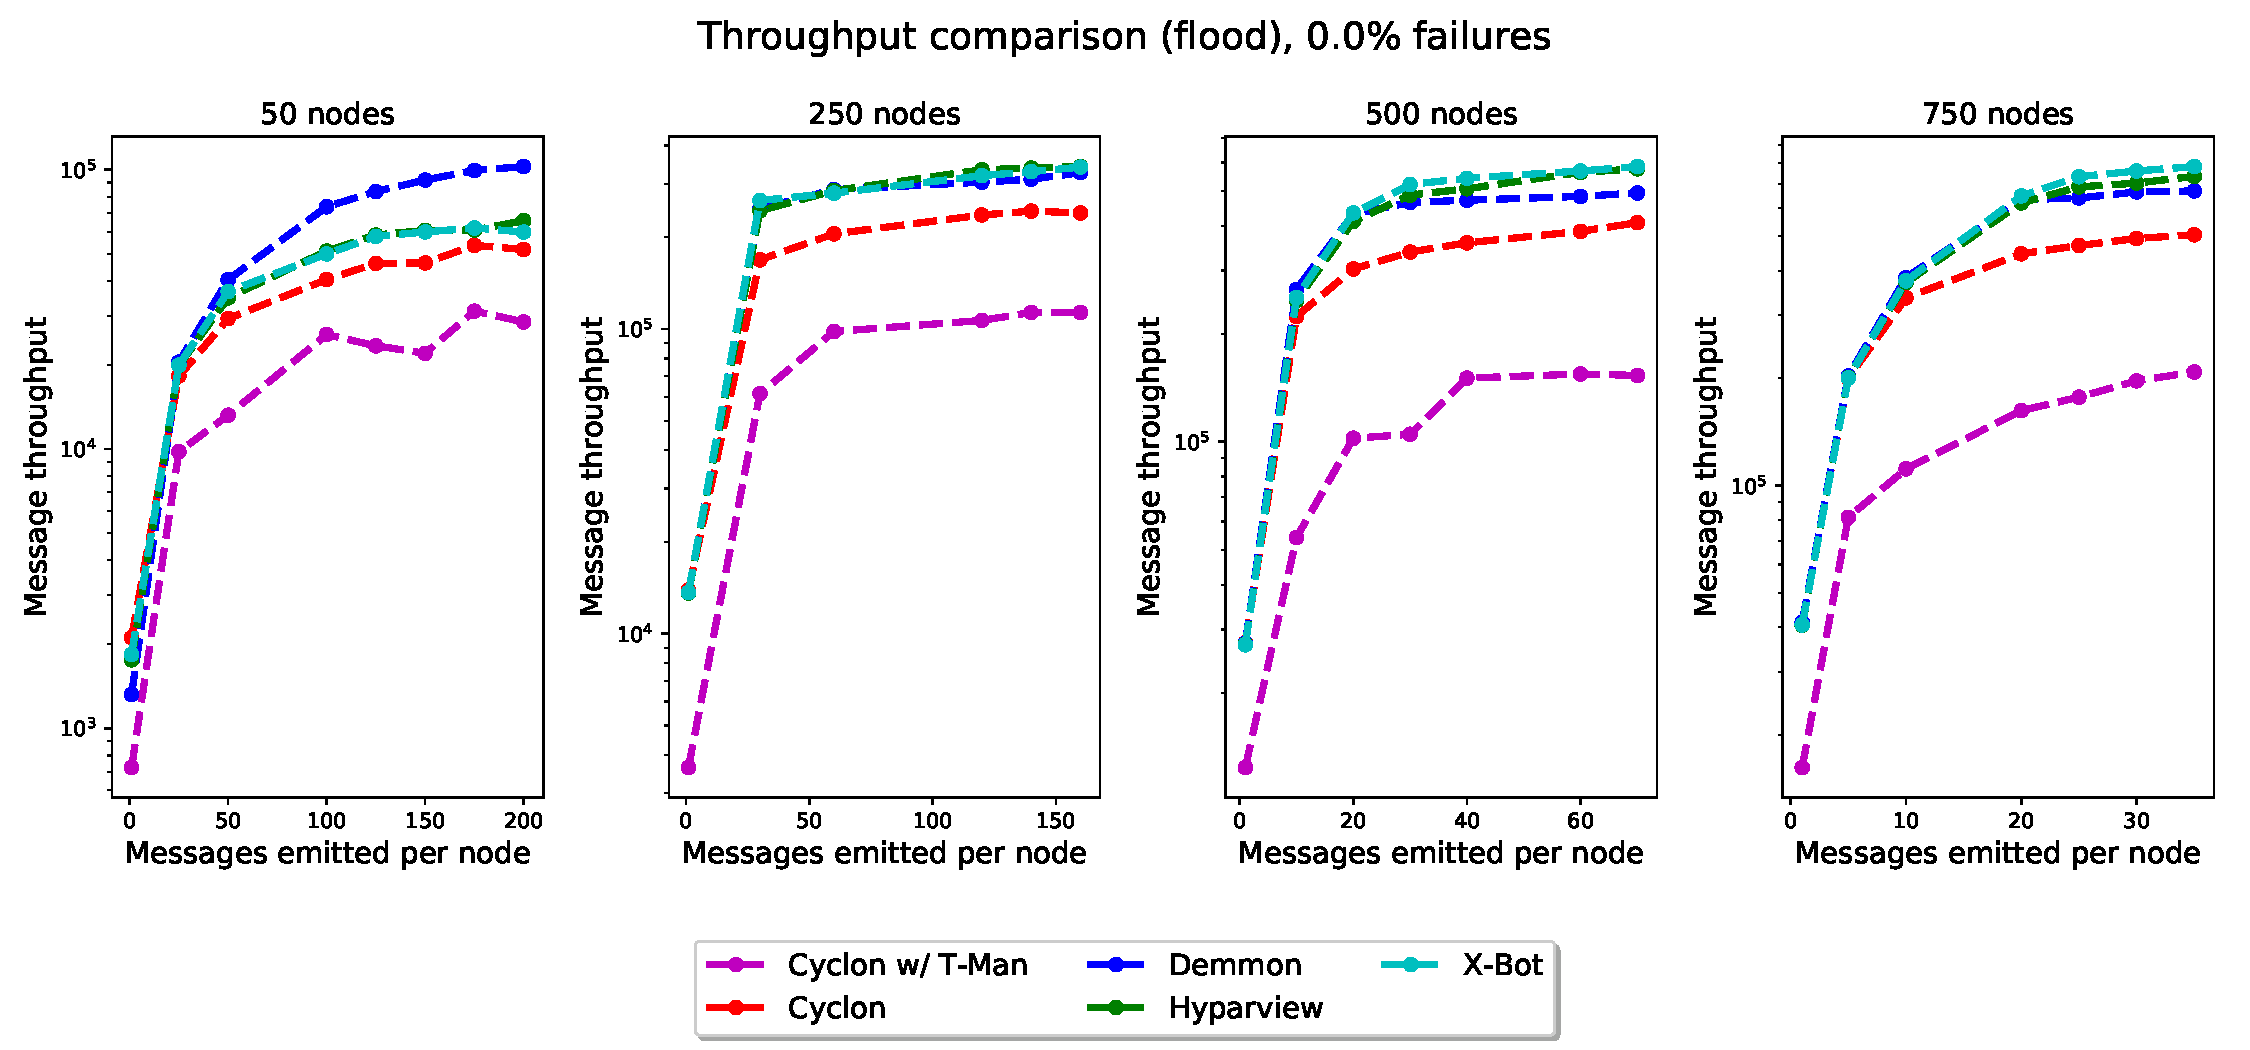
\includegraphics[width=\linewidth]{Chapters/evaluation/figures/flood/flood_0.0_failures_throughput.pdf}
    \caption{Maximum message throughput during experiment (30 second window) in simple flood scenario (0\% failures)}
    \label{fig:overlay_proto_res_msg_diss:0_failures_throughput_flood}
\end{figure}

In figure \ref{fig:overlay_proto_res_msg_diss:0_failures_throughput_flood}, we may observe the obtained throughput across the simple flood experiments with 0 failures, as we can observe, in lower node counts, the throughput achieved by deMMon surpasses the throughput achieved by the remaining protocols on lower node counts (i.e. 50 nodes), which also explains the higher values of reliability achieved by deMMon in these node counts (see fig. \ref{fig:overlay_proto_res_msg_diss:50_failures_reliability_flood}). However, at higher node counts, all protocols tend to plateau at the same throughput, which we believe to be attributed to the fact that, as previously mentioned, the tradeoffs of using a tree (a single node possibly becoming a bottleneck for many other nodes in the system) tends to impact the system the same amount that sending multiple redundant messages does.


\begin{figure}[htbp]
    \centering
    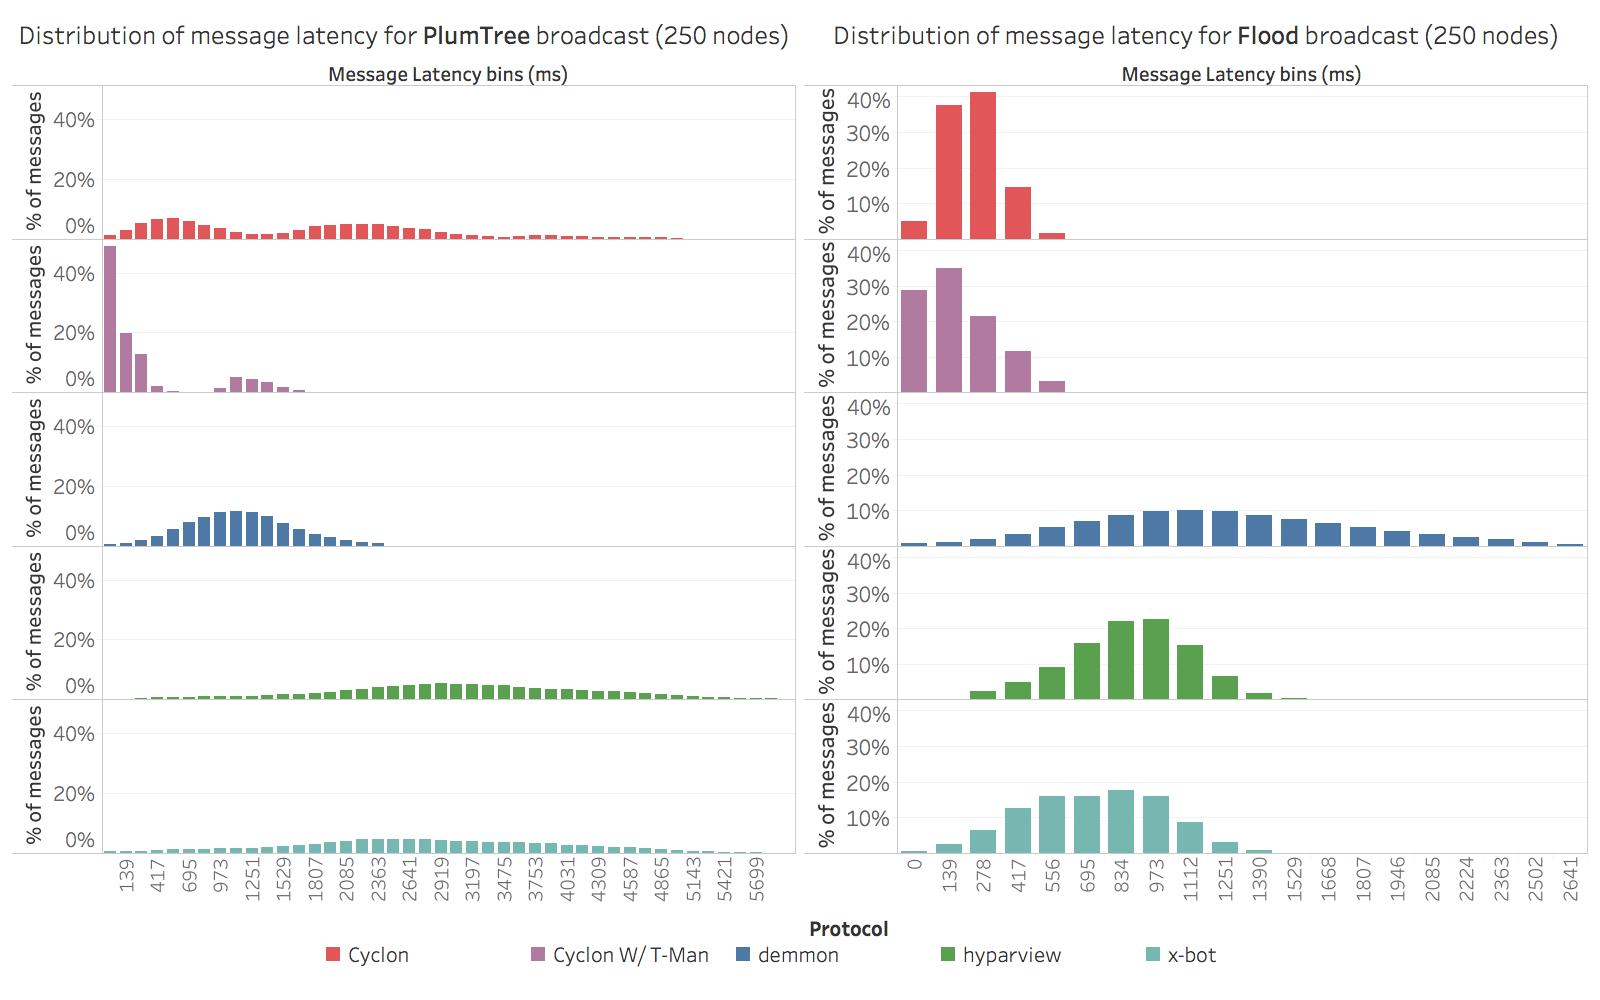
\includegraphics[width=\linewidth]{Chapters/evaluation/figures/flood/Message latency comparison.jpg}
    \caption{Message latency distribution in scenario with low network saturation}
    \label{fig:overlay_proto_res_msg_diss:0_failures_msg_lat_histogram}
\end{figure}


\begin{figure}[htbp]
    \centering
    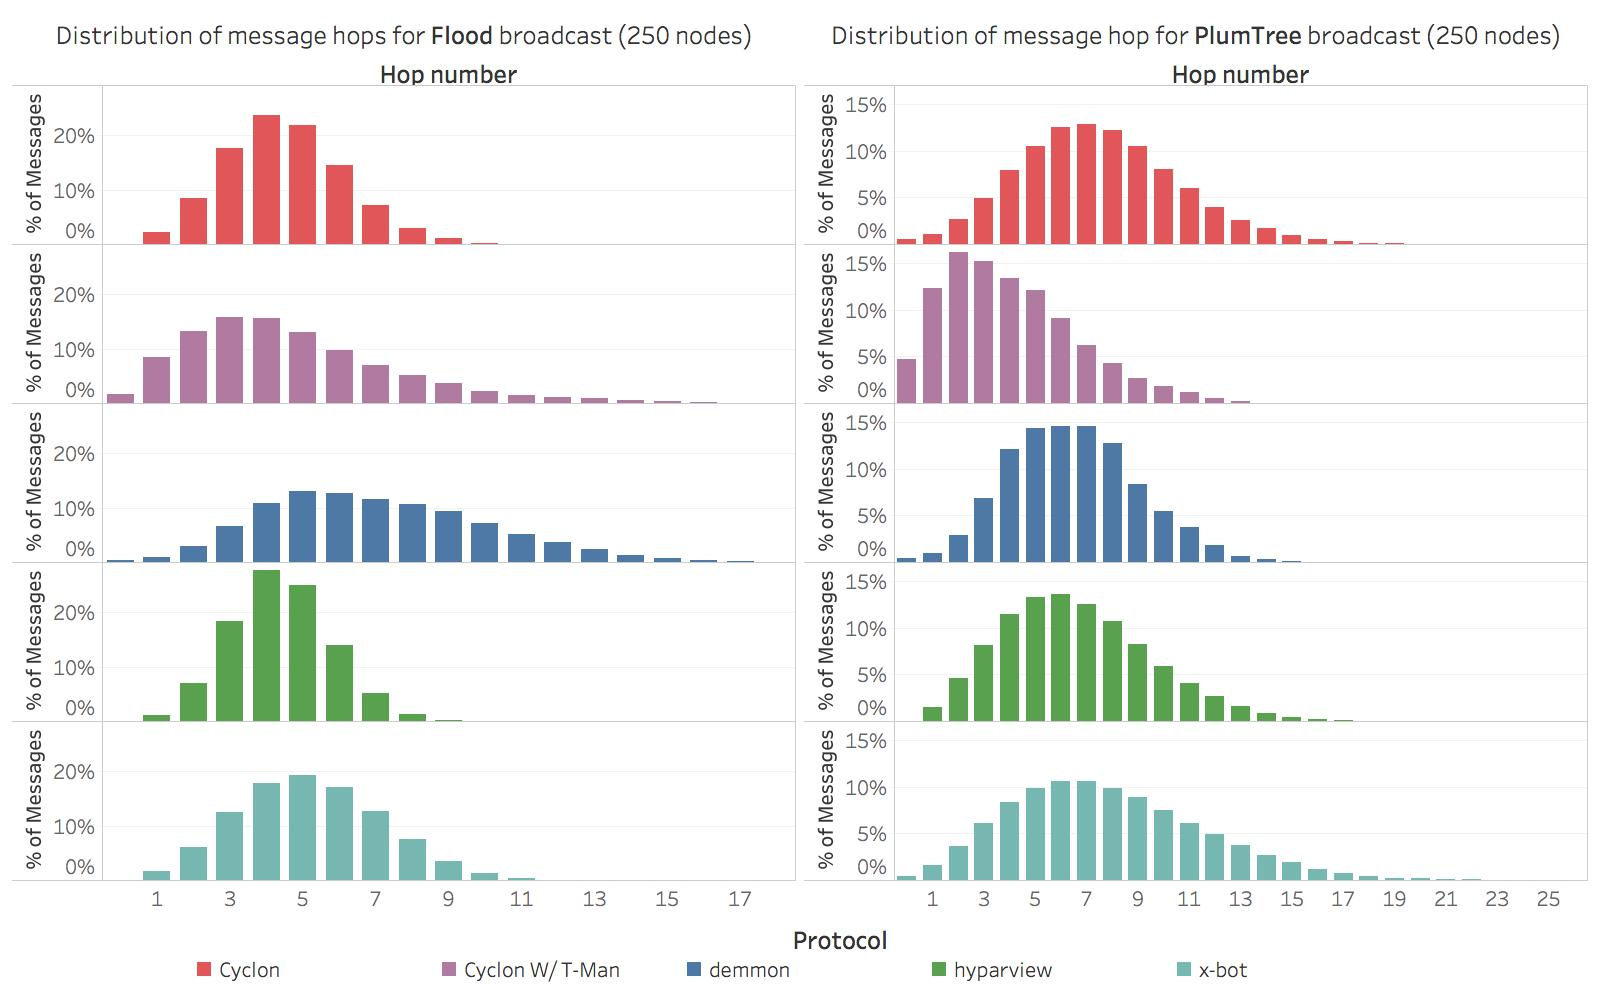
\includegraphics[width=\linewidth]{Chapters/evaluation/figures/flood/Message hop distribution.jpg}
    \caption{Message hop distribution in scenario with low network saturation}
    \label{fig:overlay_proto_res_msg_diss:0_failures_msg_hop_histogram}
\end{figure}

In figure \ref{fig:overlay_proto_res_msg_diss:0_failures_msg_lat_histogram} we compare the baseline protocols with DeMMon in regard to the message latency. These results show the averaged latency distribution for the tests conducted with 250 nodes and 1 message emitted per node. In the left we may observe the results obtained by the execution of PlumTree with the baseline protocols, while in the right we have the results for the simple flood tests. As we can observe, in general, the message latency obtained by combining simple flood with the baseline protocols tends to be lower in latency when compared with protocols that employ shared trees to disseminate the messages, such as PlumTree and DeMMon. We believe this can be explained by the fact that, by employing a single shared tree to disseminate the messages, as the messages must take specific routes in the broadcast procedure in order to decrease message redundancy, messages have to take more hops to get to their destination, consequently achieving higher latency values. This behaviour is observable in figure \ref{fig:overlay_proto_res_msg_diss:0_failures_msg_hop_histogram}, which shows the hop distribution of the delivered messages in the same scenario of 250 nodes and 1 message emitted per node.

It is important to mention that, while cyclon with T-Man achieves lower latency values in both tests, it does so at the cost of reliability, making it less applicable for a reliable broadcasting solution (as observable in the graphs displayed in \ref{fig:overlay_proto_res_msg_diss:0_failures_reliability_flood} and \ref{fig:overlay_proto_res_msg_diss:0_failures_reliability_plumTree}.


\subsection{Summary}

In this section we covered the obtained results from experimental evaluation of the devised membership protocol against multiple popular baseline protocols obtained from the study of the state of the art. Two main aspects of the devised protocol were tested at multiple scales: the first aspect was was the ability to establish and maintain the overlay connections, where results show that the devised protocol is consistently the fastest protocol to converge to a final topology. Furthermore, in regard to the latency values of the vertical connections of the established tree (excluding connections between nodes sharing the same parent in the tree, which are less used in general), DeMMon also achieves both the lower average and total latency cost.

The second tested aspect of the devised protocol was their message dissemination capacity, where the devised protocol was evaluated against the previously mentioned benchmarks paired with two flood protocols: a simple flood and the PlumTree protocol. We conducted tests at both multiple scales and multiple failure rates and observed that while DeMMon tends to perform particularly well in regard to throughput at lower scales (50 nodes) when compared with any other tested protocol, while at larger scales its throughput tends to plateau at around the values as both X-Bot and Hyparview when paired with simple flood. We also observed that, while tree topologies (both deMMon and PlumTree) incur lower message redundancy, the use of a single shared tree for scenarios with multiple senders causes higher delays in messages when compared to the simple flood alternative, which is caused by messages taking more hops to reach their destination.

To conclude, we believe to have built an overlay protocol that performs competitively with popular solutions from the state of the art for performing information dissemination. The conducted tests suggest that DeMMon performs particularly better for saturation tests at lower node counts, indicating it as the most performant solution for these scenarios. However, for scenarios where message latency is a concern, results show that any tree approach (including DeMMon), performs worse when compared to simple flood protocols.

% We now discuss the remaining obtained results from testing the baseline protocols executing a simple flood protocol against deMMon, beggining with the obtained latency values for the scenario with no failures, detailed in figure \ref{}. 

% \newgeometry{margin=1cm}
%     \begin{landscape}
%         \thispagestyle{empty}
%         \begin{figure}
%             \centering
%             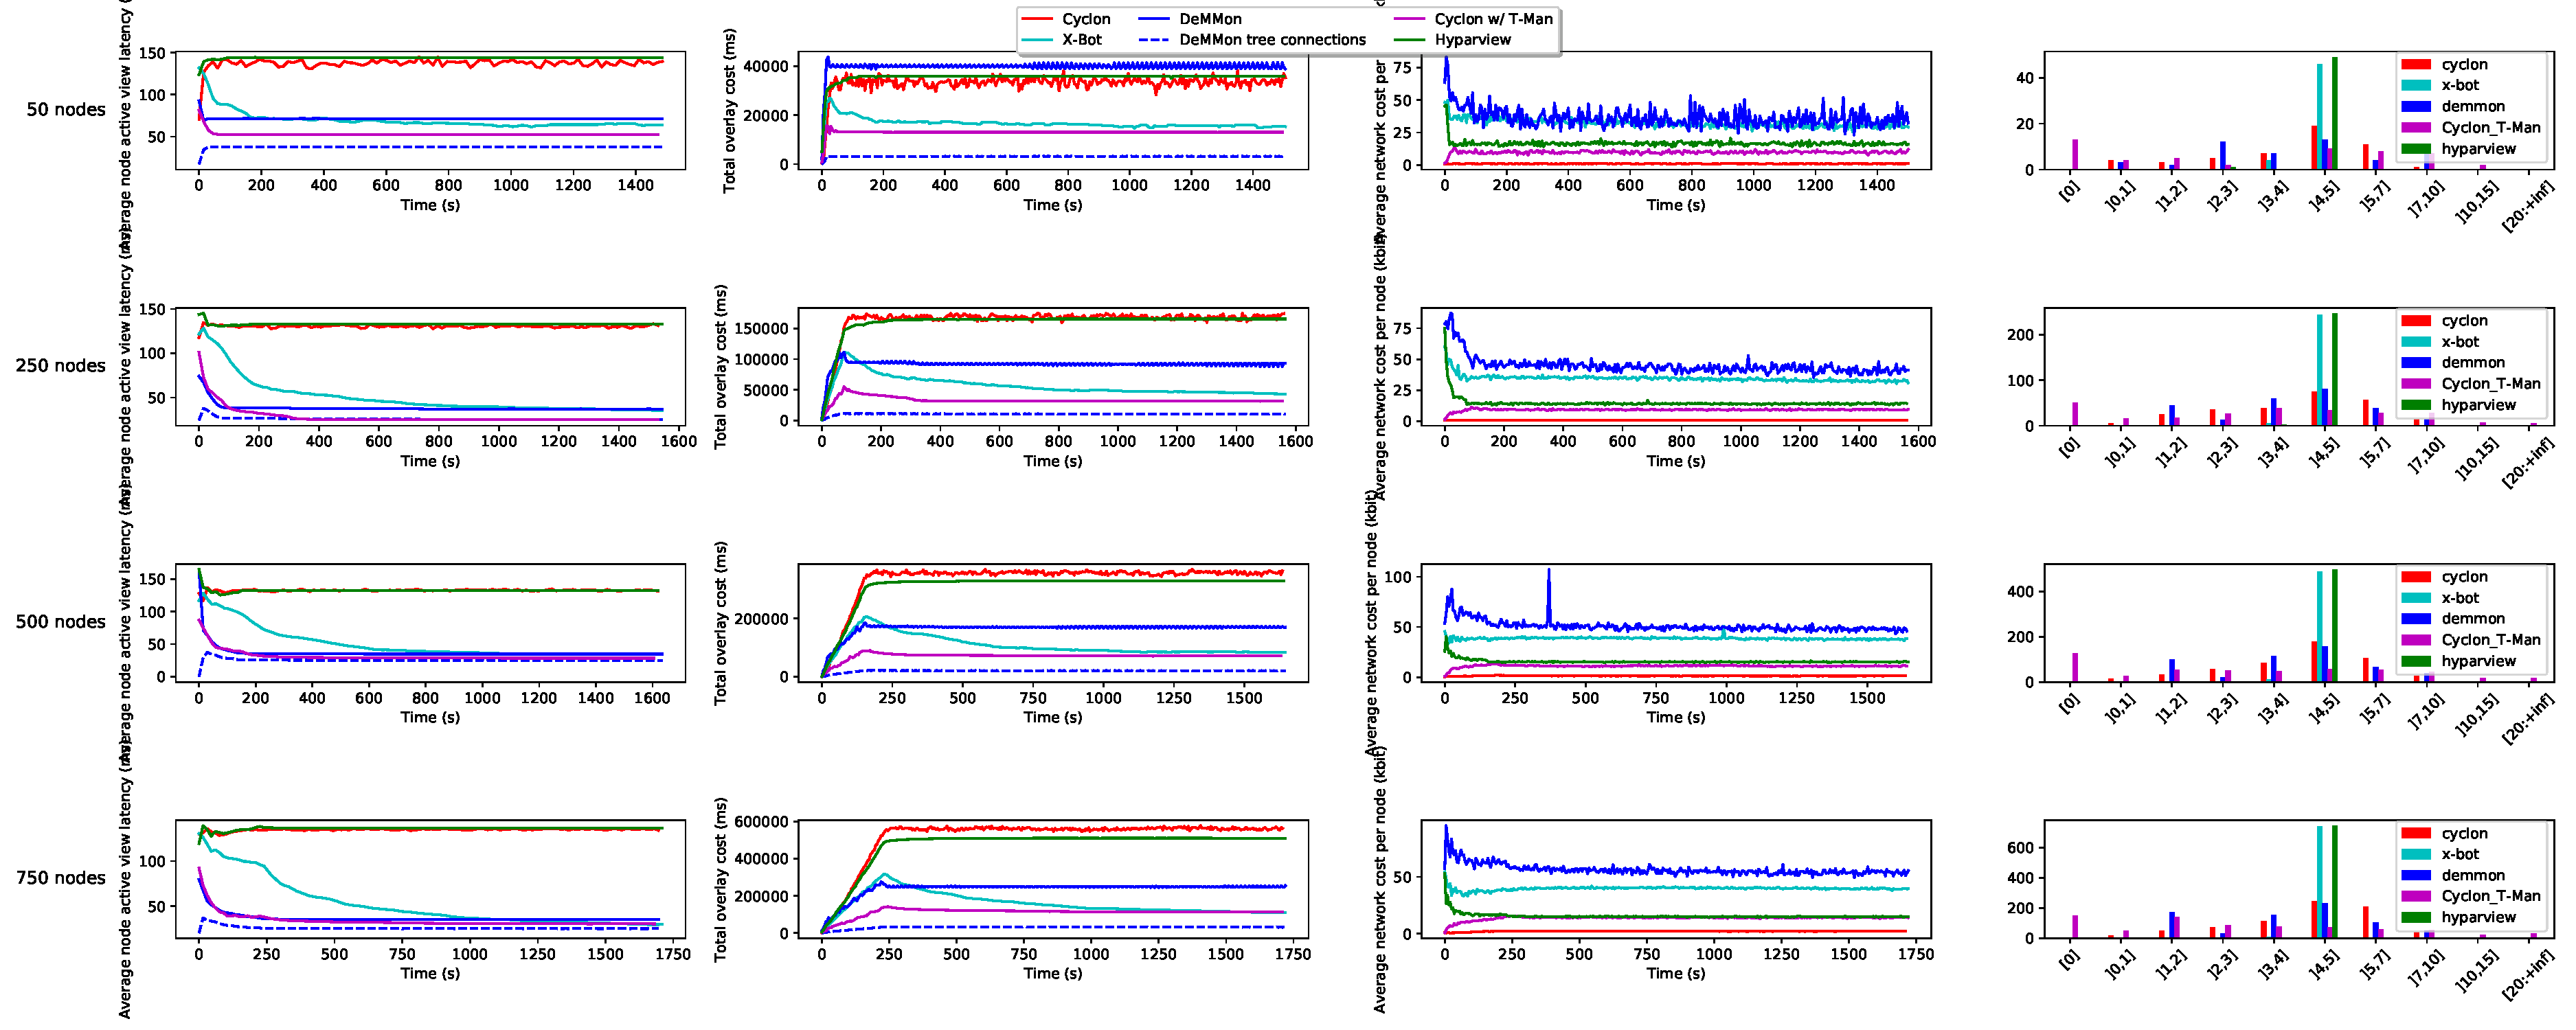
\includegraphics[width=\linewidth]{Chapters/evaluation/figures/membership_0_failures.pdf}
%             \caption{Overlay protocol comparison with failures 0 failures for network sizes of 50, 250, 500 and 750 nodes.}
%             \label{fig:overlay_proto_res_net_building:0_failures}
%         \end{figure}
%     \end{landscape}
% \restoregeometry

% \newgeometry{margin=1cm}
%     \begin{landscape}
%         \thispagestyle{empty}
%         \begin{figure}
%             \centering
%             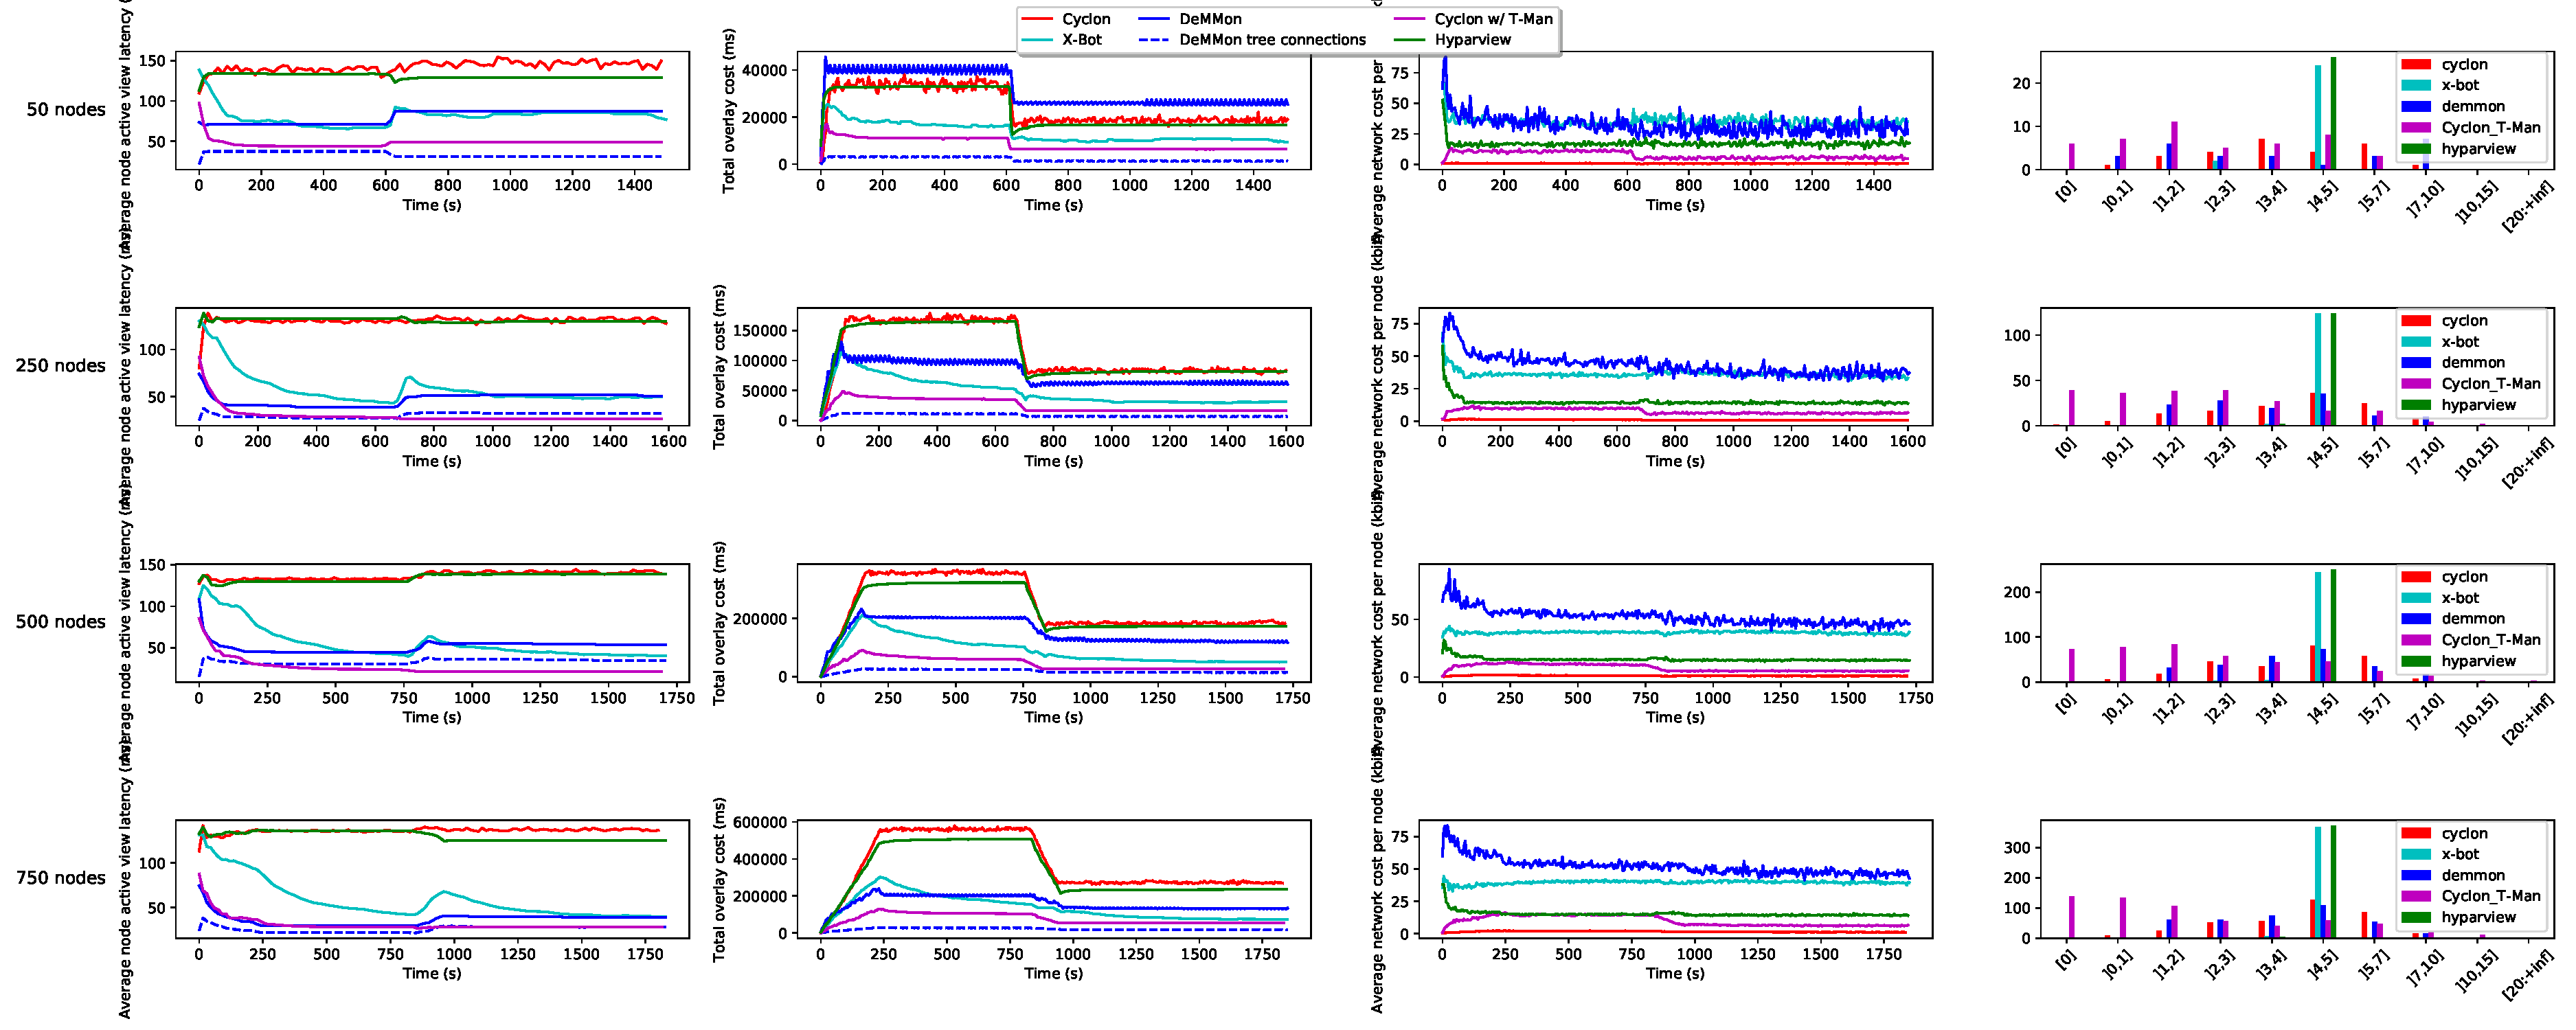
\includegraphics[width=\linewidth]{Chapters/evaluation/figures/membership_50_failures.pdf}
%             \caption{Overlay protocol comparison with failures 50\% failures for network sizes of 50, 250, 500 and 750 nodes.}
%             \label{ig:overlay_proto_res_net_building:50_failures}
%         \end{figure}
%     \end{landscape}
% \restoregeometry
